%             Exemple d'utilisation de la classe thesul
%             ------------------------------------------
%
%
% (de manière generale, les commandes de thesul sont celles
% qui ne sont pas complètement en minuscules)
%
% Voir la documentation complète pour plus de détails.
%   
%
% D. Roegel, 30 mars 2013
%
% \documentclass[12pt, oneside]{TUL/thesul}
\documentclass[12pt]{TUL/thesul}
%----------------------------------------------------------------------
%                     Chargement de quelques packages
%----------------------------------------------------------------------

% Si l'on veut produire une version PDF avec des hyperliens :
% \usepackage[pageanchor=false]{TUL/tulhypref}
% \usepackage[hidelinks, pdftex]{TUL/tulhypref}
\usepackage[hidelinks]{TUL/tulhypref}
% \usepackage[sc]{mathpazo}
\linespread{1.0}
% Si on veut le style de bibliographie named :
%\usepackage{named}

% Pour les figures :
\usepackage{graphicx}

% Si on veut des mini-tables des matières (utiliser minitoc-hyper 
% en conjonction avec tulhypref) :
\usepackage[french]{minitoc}

\usepackage{titlesec}
\usepackage{url}
\usepackage{listings}
\usepackage{pstricks}
\usepackage{subfigure}
\usepackage{amsmath}
\usepackage{amsthm}
\usepackage{amssymb}
\usepackage{tabularx}
\usepackage{textcomp}
\usepackage{multirow}
\usepackage[algoruled,french,onelanguage,algochapter]{algorithm2e}
\usepackage[section]{placeins}
\usepackage{xcolor}
\usepackage{colortbl}

\usepackage{epstopdf}
\usepackage{graphicx} % pour insérer des images
\usepackage{stmaryrd}
\usepackage{amsfonts}
% \usepackage{tikz}
% \usepackage{tikz-qtree}
% les figure imbriquées
\usepackage{epsfig}
% \usepackage{enumerate}

\usepackage{pgf}
\usepackage{tikz, calc}
% \usepackage{tikz-cd}
\usetikzlibrary{positioning}
\usetikzlibrary{fit}
\usetikzlibrary{shapes.multipart,calc}
\usetikzlibrary{arrows}

% \usepackage[math]{iwona} 
% \usepackage{iwona} 
% \SetMathAlphabet{\mathtt}{iwona}{OT1}{\ttdefault}{m}{n}

\usepackage[backend=biber, language=french, maxnames=5, citestyle=alphabetic,bibstyle=alphabetic,backref,abbreviate=false,dateabbrev=false,isbn=false,url=false,doi=true]{biblatex}
% \usepackage[backend=biber, language=french, maxnames=5,backref,abbreviate=false,dateabbrev=false,isbn=false,url=false,doi=true]{biblatex}
\addbibresource{these.bib}
% \usepackage[font=small,skip=0pt]{caption}
\usepackage[skip=0pt]{caption}
\usepackage{etoolbox}
\usepackage{needspace}

% Todo
\newcommand{\done}[1]{\todo[color=green!80!blue!80]{#1}}
\newcommand{\idone}[1]{\todo[inline,color=green!80!blue!80]{#1}}

% Samples
\newcommand{\telock}{tELock}

% Structure
\newtheorem{pb}{Problème}
\newtheorem{theo}{Théorème}
\newtheorem{defi}{Définition}
\newtheorem{prop}{Proposition}
\newtheorem{propri}{Propriété}
\newtheorem{pr}{Preuve}
\newtheorem{cor}{Corollaire}
\newtheorem{rem}{Remarque}
% \theoremstyle{remark}\newtheorem*{preuve}{Preuve}

% % Abbreviations :
\newcommand{\helloworld}{\texttt{Hello World}}
\newcommand{\nasm}{NASM}
\newcommand{\xq}{x86}
\newcommand{\xs}{x86$\_$64}

% Adresses mémoire :
\newcommand{\adr}[1]{$#1$}

% Registres
\newcommand{\eax}{\texttt{eax}}
\newcommand{\ebx}{\texttt{ebx}}
\newcommand{\ecx}{\texttt{ecx}}
\newcommand{\edi}{\texttt{edi}}

% Instructions
\newcommand{\mov}{\texttt{mov}}
\newcommand{\cmp}{\texttt{cmp}}
\newcommand{\add}{\texttt{add}}
\newcommand{\jmp}{\texttt{jmp}}
\newcommand{\ret}{\texttt{ret}}
\newcommand{\call}{\texttt{call}}
\newcommand{\push}{\texttt{push}}
\newcommand{\jne}{\texttt{jne}}
\newcommand{\je}{\texttt{je}}
\newcommand{\sub}{\texttt{sub}}

% Sémantique statique
\newcommand{\BN}{\mathbb N}
\newcommand{\BV}{\mathbb V}
\newcommand{\BX}{\mathbb X}
\newcommand{\BA}{\mathbb A}
\newcommand{\BP}{\mathbb P}
\newcommand{\BT}{\mathbb T}
\newcommand{\BL}{\mathbb L}
\newcommand{\BB}{\mathbb B}
\newcommand{\BNB}{\mathbb N\cup\{\bot\}}
\newcommand{\PN}{\mathcal{P}(\BN)}
\newcommand{\PMN}{\mathcal{P}_M(\BN)}
\newcommand{\Trs}{\mathbb N\cup\{\bot,\top\}}
\newcommand{\TTrs}{\mathcal P(\mathbb V\rightarrow\mathbb N\cup\{\bot,\top\})}
\newcommand{\Tr}{\PN\cup{\top,\bot}}
\newcommand{\TrM}{\PMN\cup\{\top,\bot\}}
\newcommand{\si}{\sigma_{init}}
\newcommand{\specialcell}[2][c]{%
  \begin{tabular}[#1]{@{}l@{}}#2\end{tabular}}
  
% Sémantique dynamique
\newcommand{\CA}{\mathcal A}
\newcommand{\CI}{\mathcal I}
\newcommand{\CC}{\mathcal C}
\newcommand{\CR}{\mathcal R}
\newcommand{\CW}{\mathcal W}
\newcommand{\da}[1]{$\CA[#1]$}
\newcommand{\di}[1]{$\CI[#1]$}
\newcommand{\dc}[1]{$\CC[#1]$}
\newcommand{\dr}[1]{$\CR[#1]$}
\newcommand{\dw}[1]{$\CW[#1]$}


\DefineBibliographyStrings{french}{
        in = {},%
%       in = {\emph{Dans}}%
        backrefpage = {cité page},
        backrefpages = {cité pages}
}

\titleformat{\chapter}[display]
  {\bfseries\huge}
  {\filleft\Large\chaptertitlename~\thechapter}
  {1ex}
  {\titlerule\vspace{1.5ex}\filright}
  [\vspace{1ex}\titlerule]

%-------------------------------------------------------------------
%                             Marges
%-------------------------------------------------------------------

% pour positionner les vraies marges:
%\SetRealMargins{1mm}{1mm}

%-------------------------------------------------------------------
%                             En-têtes
%-------------------------------------------------------------------

% Les en-têtes: quelques exemples
%\UppercaseHeadings 
%\UnderlineHeadings
%\newcommand\bfheadings[1]{{\bf #1}}
%\FormatHeadingsWith{\bfheadings}
%\FormatHeadingsWith{\uppercase}
%\FormatHeadingsWith{\underline}
\newcommand\upun[1]{\uppercase{\underline{\underline{#1}}}}
\FormatHeadingsWith\upun

\newcommand\itheadings[1]{\textit{#1}}
\FormatHeadingsWith{\itheadings}

% pour avoir un trait sous l'en-tete:
\setlength{\HeadRuleWidth}{0.4pt}

\usepackage[disable]{todonotes}

\begin{document}
\OddHead={{\leftmark\rightmark}{\hfil\slshape\rightmark}}
\EvenHead={{\leftmark}{{\slshape\leftmark}\hfil}}
\OddFoot={\hfil\thepage}
\EvenFoot={\thepage\hfil}
\pagestyle{ThesisHeadingsII}

\mainmatter 

% \chapter{Techniques d'obscurcissement de code}
% L'analyse d'un logiciel malveillant a pour but de comprendre ses mécanismes internes : selon les logiciels il peut, entre autres, s'agir des techniques d'attaque, de communication avec le concepteur ou d'autres programmes malveillants, de clés de chiffrement utilisées. Le programmeur a donc intérêt à protéger son logiciel contre l'analyse. Son but est de la rendre plus compliquée pour nécessiter plus de ressources en temps ou en argent de la part de l'analyste.

De nombreuses techniques de protection sont applicables à un programme binaire pour rendre son analyse plus compliquée. Certaines rendent le code plus difficile à comprendre en ajoutant par exemple du code inutile. Une autre technique consiste à modifier le programme au cours de son exécution afin que le code réellement utile du binaire ne soit pas lisible à première vue : on parle alors d'auto-modification.

Un auteur de programmes malveillants peut produire dans un premier temps son programme sans protection puis utiliser un logiciel de protection ou \emph{packer} qui produit un binaire sémantiquement équivalent mais qui est rendu plus difficile à analyser. En pratique l'exécutable final, protégé, combine plusieurs techniques d'obscurcissement dont des techniques d'auto-modification.

Dans ce chapitre nous chercherons rapidement a comprendre les difficultés rencontrées pour quiconque cherche à protéger son programme contre l'analyse. Dans un second temps nous nous intéresserons aux protections rencontrées lors de l'analyse de logiciels malveillants et en particulier aux problèmes liés au chevauchement de code assembleur et à l'auto-modification.

% Nous décrivons maintenant plusieurs techniques d'obscurcissement statiques ainsi que l'auto-modification.

% $\mathcal{T}$

\section{Théorie de l'obscurcissement}
\itodo{Chaîner les protections}

Collberg et Nagra \cite{nagra2009surreptitious} définissent plusieurs propriétés souhaitables pour une protection logicielle, nous reprenons ici quelque uns de leurs arguments. La première propriété est que le programme protégé soit équivalent en terme de sorties que le programme d'origine.
Une protection, ou obscurcissement, d'un programme P est une transformation $\mathcal{T}$ telle que le programme $\mathcal{T}(P)$ a le même comportement que P : quelle que soit l'entrée I de P, $\mathcal{T}(P)(I)=P(I)$.
On souhaite également ne pas affecter de manière importante les performances du programme, que ce soit en termes de temps d'exécution ou de taille des binaires.

Afin d'évaluer l'efficacité des protections il est nécessaire de définir les actifs que l'on cherche à protéger. 
Il peut s'agir de quelques algorithmes centraux au programme, de clé de chiffrement, du nom des fonctions et des variables utilisées, etc.
Il est également utile de masquer l'utilisation de techniques de protection qui pourraient attirer l'attention lors d'une analyse antivirale. De même si l'analyste se doute que le binaire emploi des protections, il n'est pas souhaitable qu'il lui soit aisé d'identifier quelles méthodes sont employées. Ainsi dans les modifications apportées au programme il est préférable que le programme final ressemble à un programme qui aurait pu être compilé, par exemple en évitant d'utiliser des instructions exotiques rarement utilisées en pratique.


En pratique un auteur de logiciel malveillant masque les symboles utiles à l'analyse tels le nom des fonctions à la compilation. Il est utile que le vecteur de propagation réussisse à masquer qu'il est protégé, s'il l'est, pour éviter une détection prématurée par un antivirus. La charge finale et les éventuels mécanismes de communication sont eux protégés contre l'analyse.\todo{cite}

\section{Exemples d'obscurcissement}
De nombreuses techniques d'obscurcissement sont utilisées en pratique, nous en donnons quelques exemples ici.

\paragraph{Insertion de code mort.}
Insérer du non atteignable (ou code mort) peut forcer un désassembleur par parcours linéaire à se désaligner avec le code réellement exécuté et à favoriser le code mort au détriment du code légitime.
L'exemple donné en figure \ref{fig:junk_right} montre de l'assembleur avec deux octets de données placés à la suite d'un instruction \jmp. Ces deux octets aux adresses $0x08048062$ et $0x08048063$ ne sont pas atteignables. Pourtant un désassembleur linéaire (Figure \ref{fig:junk_fooled}) chercherait à les désassembler et serait alors incapable de voir une partie des instructions réellement exécutées.


\begin{figure}
\begin{lstlisting}[language={[x86masm]Assembler}, escapechar=~]
08048060    eb 02               jmp 0x8048064
08048062    0a 05		~(code non atteignable)~
08048064    83 f9 02            cmp ecx, 0x2
08048067    74 00               je 0x8048069
08048069    bb 02 00 00 00      mov ebx, 0x2 ;  0x00000002
\end{lstlisting}
\caption{Insertion de code mort dans du code légitime}
\label{fig:junk_right}
\end{figure}

\begin{figure}
\begin{lstlisting}[language={[x86masm]Assembler}, escapechar=~]
08048060    eb 02               jmp 0x8048064
08048062    0a 05 83 f9 02 74   or al, [0x7402f983]
08048068    00 bb 02 00 00 00   add [ebx+0x2], bh
\end{lstlisting}
\caption{L'insertion de code mort dupe facilement un désassemblage par parcours linéaire}
\label{fig:junk_fooled}
\end{figure}

\FloatBarrier

\paragraph{Appels de fonctions sans retour.}
L'utilisation d'un contrôle de flot non standard peut forcer un désassembleur par parcours récursif à explorer du code non atteignable. 
Le comportement par défaut de l'instruction \call\ à une adresse $a$ et de taille $n$ est d'empiler l'adresse de retour $a+n$ puis de sauter vers la première adresse de la fonction appelée.
L'instruction \ret\ placée à la fin de la fonction appelée dépile la première valeur de la pile et provoque un saut vers celle-ci.

Normalement la valeur dépilée lors du \ret\ est $a+n$ afin que le flot d'exécution revienne à la fonction appelant.
Ainsi un désassembleur récursif désassemble à partir de la cible du \call\ ainsi que de l'adresse de retour.

Une technique classique d'obscurcissement \cite{LD03}\cite{PMA} consiste à combiner l'empilement d'une adresse (\push\ $a$) et l'instruction \ret. Ces deux instructions provoquent un saut vers l'adresse $a$ sans possibilité de revenir à l'instruction suivant le \call. La transformation consiste alors à remplacer des instructions \jmp\ par la séquence \push\ puis \ret\ puisque les deux suites d'instructions suivantes sont équivalentes.
\begin{center}
\begin{tabular}{c|c}
\push\ \adr{a} & \jmp\ \adr{a}\\
\ret &
\end{tabular}
\end{center}

\paragraph{Prédicats opaques.}
% À l'instar de son comportement avec une instruction \call, 
Lorsqu'un désassembleur récursif rencontre une instruction de saut conditionnel comme \je, qui provoque un saut si les deux valeurs comparées sont égales, il cherche à désassembler à la fois la cible potentielle du saut comme l'instruction suivante, qui sera exécutée si la condition n'est pas remplie.
Une autre technique courante d'obscurcissement consiste à utiliser comme condition du saut une relation que le programmeur sait toujours vraie ou fausse \cite{MKK07}. De cette manière il prédit qu'une seule des deux branches est atteignable alors qu'un désassembleur va parcourir également la branche inutile.
Une telle condition est appelée un prédicat opaque et peut par exemple être implémentée par des relations d'arithmétique. Par exemple en appliquant le petit théorème de Fermat \cite{fermat} : quel que soit l'entier e, $e^3\ =\ e\ mod\ 3$.
Le programmeur sait que l'égalité est toujours vérifiée mais un analyseur statique ne pourra pas le déterminer aisément.

\paragraph{Applatissement de graphe de flot de contrôle.}

\section{Chevauchement de code}
\itodo{citer PMA}
\itodo{biblio + complète}
\itodo{figure telock : les octets, jolis}
On a vu que la taille d'une instruction assembleur varie de un à 15 octets \done{15 dans intel2 chercher 15}.
De plus rien n'empêche que la cible d'un saut soit une adresse se trouvant être au milieu d'une autre instruction.
Ainsi on parle de chevauchement de code lorsque deux instructions (ou plus) à des adresses différentes sont codées sur des adresses communes. Si une instruction à l'adresse \adr{a} de taille $k\geq 2$ est atteignable, il peut y avoir une autre instruction valide et atteignable à l'adresse \adr{a+1} et ces deux instructions se chevauchent.

Il est à noter que, comme indiqué par Sikorski et Honig \cite{PMA}, il n'y a dans ce cas aucun désassemblage sous forme de liste d'instructions assembleur qui soit correct puisqu'une telle liste devra choisir entre l'instruction à l'adresse \adr{a} et celle à l'adresse \adr{a+1} alors qu'elles sont toutes les deux valides et atteignables. Une solution pour écrire un tel code assembleur est de mettre la première instruction en temps qu'instruction classique tandis que la deuxième sera présente sous forme d'octets codés en dur dans le fichier assembleur.

\paragraph{Exemple dans \telock.}
Le code de la figure \ref{fig:telock_obf_disas} est extrait d'un programme protégé par \telock\ désassemblé à l'aide d'un parcours récursif à partir de l'adresse \adr{01006e7a}. Il y a une instruction \texttt{jmp +1} à l'adresse \adr{01006e7d} et codée sur les deux octets \texttt{eb ff}, qui saute vers l'adresse \adr{01006e7d+1} où est présenté l'instruction \texttt{dec ecx}, codée sur \texttt{ff c9} et qui partage donc l'octet \texttt{ff} à l'adresse \adr{01006e7d+1} avec l'instruction \jmp.

Le code assembleur permettant d'être assemblé en ces octets est donné figure \ref{fig:telock_obf_asm} : la première instruction \jmp\ peut être présente dans le code tandis que l'instruction \dec\ la chevauchant est codée en dur grâce à l'octet \texttt{c9}.

\begin{figure}
% \scriptsize
% 0x01006e73    00 0c 0b        add [ebx+ecx], cl
% 0x01006e76    80 34 0b 67     xor byte [ebx+ecx], 0x67
\begin{lstlisting}[language={[x86masm]Assembler}, escapechar=~]
01006e7a    fe 04 0b        inc byte [ebx+ecx]
01006e7d    eb ff           jmp +1
01006e7e       ff c9        dec ecx
01006e80    7f e6           jg 01006e68
01006e82    8b c1           mov eax, ecx
\end{lstlisting}
% \end{framed}
\caption{Désassemblage récursif de \telock}
\label{fig:telock_obf_disas}
\end{figure}

\begin{figure}
% \scriptsize
% 0x01006e73    00 0c 0b        add [ebx+ecx], cl
% 0x01006e76    80 34 0b 67     xor byte [ebx+ecx], 0x67
\begin{lstlisting}[language={[x86masm]Assembler}, escapechar=~]
inc byte [ebx+ecx]
jmp +1
db c9 			; ajout de l'octet c9
jg 01006e68
mov eax, ecx
\end{lstlisting}
% \end{framed}
\caption{Code assembleur du chevauchement de \telock}
\label{fig:telock_obf_asm}
\end{figure}


Le graphe de flot de contrôle correct pour ce code est donné sur la figure \ref{fig:telock_cfg}. Le sommet orange est la première instruction et les lignes en pointillés reliant deux sommets marquent un chevauchement entre les instructions de ces sommets.

\begin{figure}
\begin{center}
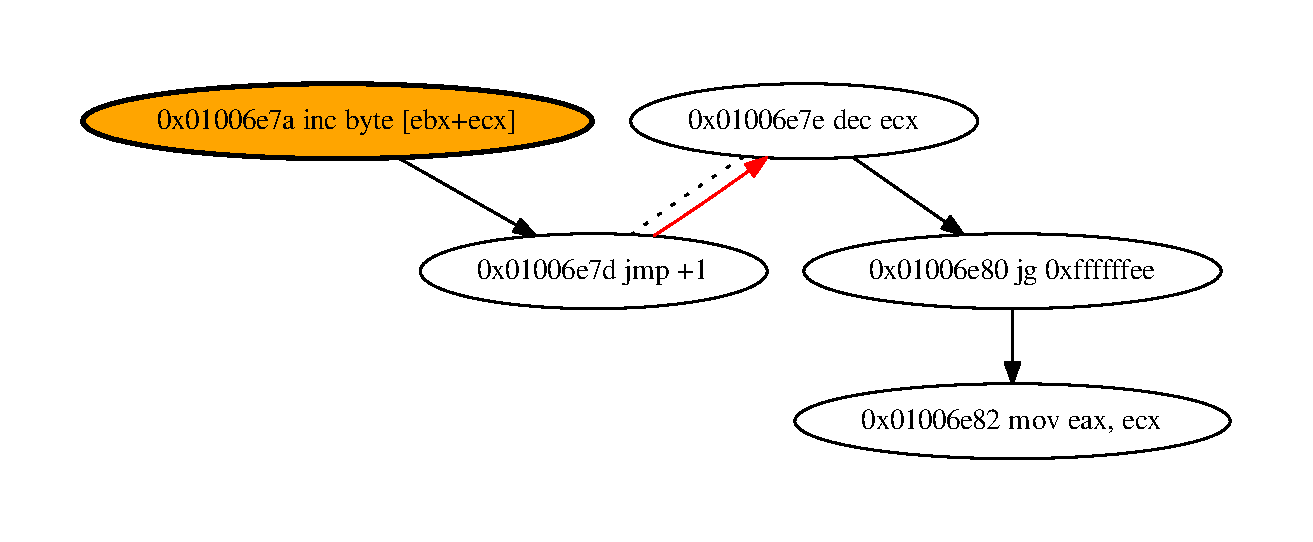
\includegraphics[width=0.8\textwidth]{supports/disasm/telock/telock.pdf}
\end{center}
\caption{Graphe de flot de contrôle de \telock}
\label{fig:telock_cfg}
\end{figure}

\paragraph{Exemple dans UPX.}

\section{Auto-modification}

% \begin{figure}
% \begin{center}
% \begin{tabular}{|l|l|l|}
% \hline
% Adresse & Octets & Instruction\\
% \hline
%  8048060  &  (...)         	& Pile -> RWX \\ 
%  804807c  &  bf 00 00 00 00         &  mov    edi, 0x0 \\
%  8048081  &  b8 91 80 04 08         &  mov    eax, 0x8048091 \\
%  8048086  &  66 c7 00 eb 00         &  mov    [eax], 0xeb \\
%  804808b  &  66 c7 40 01 07 00      &  mov    [eax+1], 0x7 \\
%  8048091  &  eb 0e                  &  jmp    80480a1 <edi3> \\
%  8048093  &  bf 01 00 00 00         &  mov    edi,0x1 \\
%  8048098  &  eb 0e                  &  jmp    80480a8 <fin> \\
%  804809a  &  bf 02 00 00 00         &  mov    edi,0x2 \\
%  804809f  &  eb 07                  &  jmp    80480a8 <fin> \\
%  80480a1  &  bf 03 00 00 00         &  mov    edi,0x3 \\
%  80480a6  &  eb 00                  &  jmp    80480a8 <fin> \\
%  80480a8  &  (...)		    &  Affiche edi \\
%  80480c3  &  (...)		    & Quitte \\
% \hline
% \end{tabular}
% \end{center}
% \caption{Exemple de code auto-modifiant}
% \label{fig:unevague_v0_code}
% \end{figure}

\begin{figure}
\begin{center}
\subfigure[Code assembleur]{
\begin{tabular}[b]{|l|l|l|}
\hline
Adresse & Octets & Instruction\\ 
\hline
 8048060  &  (...)         	& Pile -> RWX \\ 
 804807c  &  bf 00 00 00 00         &  mov    edi, 0x0 \\
 8048081  &  b8 91 80 04 08         &  mov    eax, 0x8048091 \\
 8048086  &  66 c7 00 eb 00         &  mov    [eax], 0xeb \\
 804808b  &  66 c7 40 01 07 00      &  mov    [eax+1], 0x7 \\
 8048091  &  eb 0e                  &  jmp    80480a1 <edi3> \\
 8048093  &  bf 01 00 00 00         &  mov    edi,0x1 \\
 8048098  &  eb 0e                  &  jmp    80480a8 <fin> \\
 804809a  &  bf 02 00 00 00         &  mov    edi,0x2 \\
 804809f  &  eb 07                  &  jmp    80480a8 <fin> \\
 80480a1  &  bf 03 00 00 00         &  mov    edi,0x3 \\
 80480a6  &  eb 00                  &  jmp    80480a8 <fin> \\
 80480a8  &  (...)		    &  Affiche edi \\
 80480c3  &  (...)		    & Quitte \\
\hline
\end{tabular}
\label{fig:unevague_v0_code}
}
\subfigure[Graphe de flot de contrôle]{
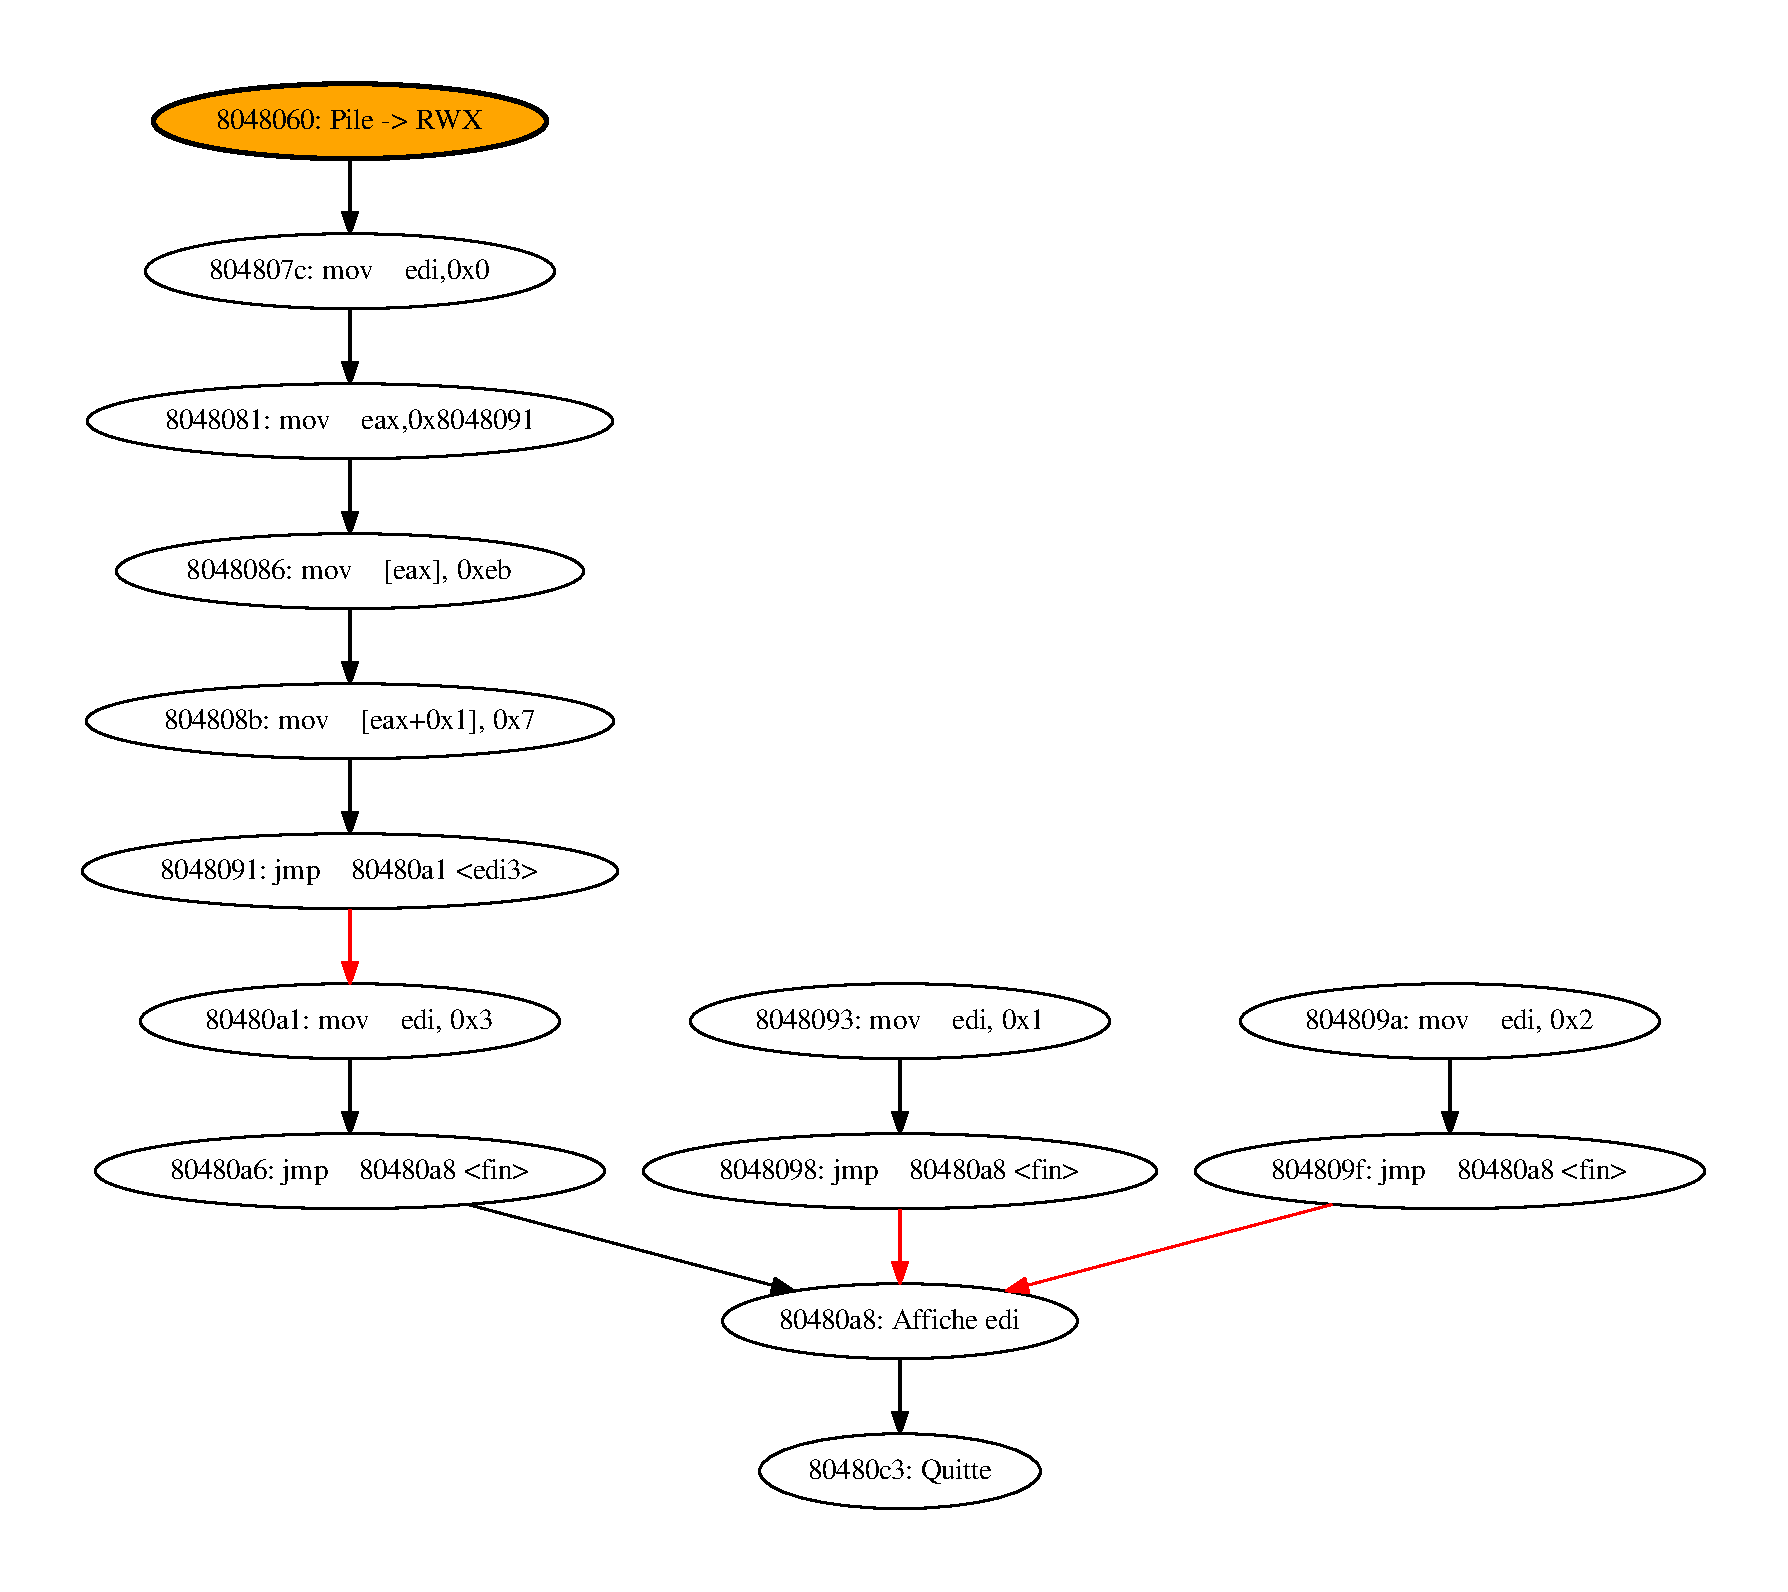
\includegraphics[width=1.0\textwidth]{supports/unevague/uv.pdf}
\label{fig:unevague_v0_cfg}
}
\end{center}
\ijym{détailler les ... (en annexe?)}
\ijym{fonction f, adresses f, f+1, f+3, ...}
\caption{Code assembleur auto-modifiant}
\label{fig:unevague_v0}
\end{figure}

Il a été expliqué dans la section \ref{section:assembleur} que, avec l'architecture de Harvard modifiée, le code n'est pas physiquement séparé des données lors de l'exécution sur une machine réelle.
Un programme auto-modifiant est simplement un programme utilisant cette propriété pour modifier le code assembleur le définissant au cours même de son exécution.
Ainsi on parle de comportement auto-modifiant lorsqu'une instruction du programme est codée sur au moins un octet qui a au préalable été modifié par ce programme.

En pratique les processeurs récents implémentent une protection, appelée bit NX ou W\textasciicircum X (prononcé ``W xor X''), permettant d'empêcher qu'une page mémoire puisse être à la fois écrite et exécutée lors de l'exécution du programme.
Cette protection a été ajoutée pour éviter des attaques résultant en l'exécution de code dans des données écrites par l'utilisateur du programme et non pour interdire l'auto-modification qui a des cas d'utilisation légitimes.
De ce fait l'activation ou non de la protection est spécifiée lors de la compilation et si un programme n'est pas protégé il lui suffit d'utiliser un appel système (\texttt{mprotect} sous linux) pour autoriser l'exécution de code sur la pile.

Prenons le programme de la figure \ref{fig:unevague_v0_code}. Ce programme commence par autoriser l'accès en écriture à la la section de code \ptext\ puis écrit sur la pile, modifie la valeur du registre \edi\ et termine par l'affichage de la valeur de \edi.
Si on ne prend pas en compte l'écriture sur la pile, il semble évident au vu du graphe de flot de contrôle (Figure \ref{fig:unevague_v0_cfg}), vu que la première instruction de saut provoque un saut vers l'instruction \texttt{mov edi,0x3} et que la seconde provoque l'affichage de \edi, que la valeur finale du registre est 3.
Pourtant les instructions \texttt{mov [eax],0xeb} et \texttt{mov [eax+1],0x07} aux l'adresse $0x8048086$ et $0x804808b$ remplacent le saut initial par un saut vers l'adresse $0x8048098$ où la valeur de \edi\ sera fixée à 2 avant l'affichage de celle-ci.


On constate ici que le programme se modifie au cours de son exécution et donc
\begin{itemize}
 \item On ne peut pas se contenter de la représentation d'origine du programme pour l'analyser.
 \item Le graphe de flot de contrôle initial peut être amené à évoluer au cours de l'exécution du programme.
\end{itemize}

\section{Logiciels malveillants et obscurcissement}
\itodo{packers, comment chaîner les obfuscations}
\itodo{utiliser des petites variations d'un packer pour éviter la détection, parler de la détection}

\section{Conclusion}
Cette thèse s'intéresse particulièrement à l'analyse des programmes écrits en assembleur \xq\ et \xs. Ces programmes ont en général été compilés à partir d'un langage de haut niveau puis ont été modifiés à l'aide d'un logiciel de protection. Les binaires que l'on étudie sont donc protégés avec des techniques statiques comme auto-modifiantes. Notre travail consiste alors à chercher à désassembler correctement ces programmes dans le but de faciliter leur analyse.

Les chapitres suivants détailleront plusieurs techniques d'analyse que nous avons appliquées. Nous nous intéresserons d'abord à l'aspect auto-modifiant des programmes et verrons comment l'analyse dynamique peut être utilisée pour reconstruire un modèle pour le programme auto-modifiant. Dans un second temps nous introduiront des techniques d'analyse statiques pour chercher à recomposer le maximum de code assembleur du programme et contourner d'autres méthodes de protection comme le chevauchement de code.

% \DontFrameThisInToc
% \chapter*{Introduction\label{chap:introduction}}
% % \section{Contexte et enjeux}
% \todo[inline]{Ajouter:
% Attaque -> Malware\\
% Marché des vulnérabilités, des malwares\\
% }
% Un logiciel opérant sur un ordinateur est dit malveillant s'il réalise volontairement des opérations allant à l'encontre de l'intérêt de l'utilisateur et ce à l'insu de celui-ci.
Un logiciel malveillant réalise volontairement des opérations allant à l'encontre de l'intérêt de l'utilisateur. 
Certaines de ces actions peuvent être objectivement malveillantes comme c'est le cas avec Stuxnet qui vise des éléments d'un système de contrôle industriel afin de le rendre inutilisable. 
% Les administrateurs utilisent quotidiennement des programmes de gestion de machine à distance. 
Un logiciel malveillant visant à fournir à un attaquant un accès à distance ne diffère pas fondamentalement, en termes de fonctionnalités, d'un logiciel légitime utilisé par un administrateur.
La différence entre les deux est que l'administrateur n'est pas au courant de l'installation du logiciel malveillant et ne peut pas le contrôler.
Nous proposons donc la définition suivante pour un logiciel malveillant.
\\

\textit{Un logiciel est dit malveillant s'il réalise volontairement des opérations allant à l'encontre de l'intérêt de l'utilisateur, et ce à l'insu de celui-ci.}
\\ 

Les actions malveillantes peuvent être de différentes natures. On parle d'atteinte à la confidentialité lorsque des données privées sont obtenues par l'attaquant, d'atteinte à l'intégrité lorsque de l'information présente sur le système attaqué est altérée par l'attaquant et d'atteinte à la disponibilité du système si l'attaquant rend le système inutilisable ou plus difficile à opérer.

Les logiciels malveillants s'attaquent en général à la confidentialité et la disponibilité du système bien que les outils d'administration à distance soient capables, une fois la machine infectée, d'attaquer les trois aspects de la sécurité de la machine.

Ainsi, en général, un logiciel malveillant diffère d'un logiciel légitime en ce qu'il cherche à dissimuler son existence et son action sur le système. Il déploie à cette fin des techniques de protection logicielles rendant son analyse plus difficile que celle du programme légitime.
On parle alors de \emph{charge utile} pour désigner l'action finale d'une attaque sur le système compromis. L'attaquant cherche à progresser dans le réseau en propageant son attaque tout en dissimulant la charge finale à des analystes éventuels.


\section*{Détection de logiciels malveillants}
Les premiers travaux traitant de virologie informatique datent de 1986 avec Cohen \cite{Cohen86} puis Adleman \cite{Adleman88} en 1988. Ils s'intéressent particulièrement au comportement auto-reproducteur de certains programmes. Déterminer si un programme a un comportement auto-reproducteur est un problème indécidable. De même il n'existe pas de programme capable de décider, sans jamais se tromper, si un programme analysé a un comportement malveillant.

Les décennies qui ont suivi ont vu apparaître différentes techniques de détection partielles dont la plus répandue est l'analyse de signatures syntaxiques. Les approches par signatures consistent dans un premier temps à extraire des caractéristiques d'un corpus de logiciels connus pour être malveillants : la présence de certaines chaînes de caractères dans le fichier contenant le programme ou l'utilisation de certaines instructions dans un ordre précis, par exemple. Dans un second temps, pour classifier un logiciel inconnu, on regarde s'il possède une des caractéristiques extraites du corpus.
Cette technique possède le double avantage d'être rapide et de générer peu de fausses alarmes.

Cependant chaque souche originale d'un logiciel malveillant est généralement déclinée en de nombreuses versions dont les fonctionnalités varient. Ces souches forment une famille de logiciels malveillants. Pour éviter la détection par signatures syntaxiques, il suffit souvent d'insérer du code inutile ou de réorganiser le code : le nouveau logiciel malveillant est identique fonctionnellement au code initial mais les signatures précédemment extraites n'y sont plus présentes.

Nous nous sommes alors intéressés à la technique de détection initiée par Kaczmarek \cite{BKM08} lors de sa thèse. Il s'agit d'une technique de détection par signatures basée sur la comparaison de graphes de flots de contrôles, c'est à dire du graphe structurant l'exécution du logiciel.
% \todo[inline]{exemple prog ->  CFG}

Dans la pratique, les logiciels malveillants sont souvent protégés par une technique d'encapsulation cachant complètement la charge utile à un analyste.
Aucune technique basée sur une observation passive du programme à analyser ne peut permettre de prédire le programme encapsulé et donc de détecter s'il est malveillant.

Afin de lutter contre différentes techniques d'obscurcissement, nous avons travaillé sur une méthode d'analyse hybride.
Dans un premier temps nous exécutons le programme pour lui faire décompresser les parties encapsulées. Dans un second temps nous analysons statiquement les parties non exécutées dans lesquelles nous identifions d'autres méthodes d'obscurcissement et y effectuons une détection.

\section*{Problèmes de recherche}
La principale difficulté lors de l'analyse d'un logiciel malveillant est qu'il est auto-modifiant : un programme encapsulé se décompresse en réécrivant sur lui-même en mémoire. L'auto-modification complexifie grandement la sémantique du programme puisqu'une instruction peut-être amenée à être modifiée au cours de l'exécution de celui-ci.

% \begin{pb}
%  Définir une sémantique et une technique d'analyse compatible avec l'auto-modification.
% \end{pb}

Afin de comprendre cette technique il est nécessaire d'utiliser une sémantique compatible avec l'auto-modification.
Nous avons repris les sémantiques définies par Reynaud \cite{Reynaud2010} et Calvet \cite{Calvet2013} séparant l'exécution d'un programme auto-modifiant en vagues. Chacune des vagues représente une étape d'exécution dans laquelle le programme n'est pas modifié. Cette représentation permet d'analyser chaque vague indépendamment des autres et d'articuler l'analyse d'un programme autour d'une trace d'exécution particulière.
Nous avons implémenté un émulateur de code \xq\ auto-modifiant : il est capable de reconstruire les vagues de la trace émulée.

% La contribution de cette thèse réside dans une sémantique et un algorithme permettant une analyse bornée de toutes les traces d'exécution possibles d'un programme. 

Nous avons ensuite cherché à désassembler un programme obscurci. Le but est de déterminer l'ensemble du code atteignable en étant à la fois correct (on doit couvrir tout le code potentiel) et précis (le code désassemblé doit pouvoir être exécuté). 

\begin{pbb}
 Désassembler et reconstruire le graphe de flot de contrôle d'un programme obscurci.
\end{pbb}

Puisque notre objectif est de comparer les graphes de programmes connus et inconnus, nous utilisons le désassemblage pour reconstruire un graphe de flot de contrôle du programme analysé.
Notre contribution est la définition et l'implémentation d'un désassembleur hybride partant d'une trace d'exécution et permettant de reconstruire le graphe de flot de contrôle de chacune des vagues du binaire à l'aide d'une analyse statique.

Enfin la comparaison des graphes de flot de contrôle, ou analyse morphologique, consistait en la détection d'isomorphismes de graphes entre des parties des graphes de flot considérés. 
L'algorithme utilisé à l'origine fonctionnait par reconnaissance d'arbres à l'aide d'un automate d'arbres. Il n'existait pas de cadre formel définissant les objets détectés par cette analyse. Sans cadre formel il était difficile de mesurer les performances des implémentations utilisées en termes de précision des résultats.

\begin{pbb}
 Formaliser et optimiser la reconnaissance de graphes dans l'optique de la détection de programmes malveillants.
\end{pbb}

Notre travail a permis de dégager la notion de site. Les sites sont des sous-graphes particuliers du graphe de flot de contrôle et sont l'entité atomique que nos algorithmes de détection d'isomorphismes cherchent à faire correspondre entre plusieurs programmes à analyser. Nous avons élaboré un algorithme correct et rapide pour des petites bases de logiciels malveillants ainsi qu'un algorithme sous-optimal mais donnant de bons résultats et dont le temps d'exécution ne dépend pas de la taille de la base.

\section*{Contributions}
Nous avons contribué à l'analyse de programmes obscurcis de deux manières.
D'une part nous avons décrit un langage assembleur disposant d'une sémantique concrète compatible avec l'exécution de programmes auto-modifiants.
Nous avons étendu BAP, une plateforme d'analyse de binaires existante, pour lui permettre d'évaluer des programmes auto-modifiants. Nous avons également formalisé le problème du chevauchement de code et étudié l'usage que les programmes obscurcis font de cette méthode de protection.
D'autre part nous avons proposé une technique de désassemblage consistant à effectuer une analyse dynamique que l'on complète à l'aide de techniques d'analyse statique. Cette technique a pour objectif de reconstruire un graphe de flot de contrôle dont nous avons défini la forme idéale.

Nous avons également contribué à l'analyse morphologique en formalisant le sous-problème d'isomorphisme de sous-graphes qu'elle cherche à résoudre. Nous avons développé et implémenté un algorithme correct et plus rapide que les approches précédentes pour résoudre ce problème ainsi qu'un algorithme incorrect mais de temps d'exécution constant.
Nous avons enfin proposé une application de la technique d'analyse morphologique au domaine de la détection de similarités logicielles \cite{REAT12,mal13} et démontré la technique sur quelques logiciels malveillants spécifiques \cite{sstic13,mal13}.


\section*{Organisation du document}

Nous commencerons, dans une première partie, par définir les notions d'assembleur et de désassemblage qui seront utilisées dans la suite du manuscrit, puis détaillerons une technique d'analyse statique, puis dynamique de programmes obscurcis. Cette partie se terminera par la combinaison des deux approches et la présentation de notre outil de désassemblage.

La seconde partie portera plus particulièrement sur l'analyse morphologique et les algorithmes de comparaison de graphes. Nous reviendrons sur les applications d'une telle méthode à la détection de programmes malveillants, à la détection de librairies logicielles et à l'analyse pratique de programmes malveillants avec l'exemple de \duqu\ et \stux.

% 
% % \WriteThisInToc
% % \FrameThisInToc
% % \NumberThisInToc
% \part{Désassemblage et analyse de binaires}
% 
% % \NumberThisInToc
% \DontFrameThisInToc
% \chapter{Assembleur\label{chap:assembleur}}
% Cette partie est consacrée à l'analyse d'un programme utilisant des méthodes de protection.
Dans ce chapitre nous expliquons dans un premier temps ce qu'est un programme binaire et les spécificités du langage assembleur dans lequel ces programmes sont écrits.
Dans un second temps nous définissons les objectifs de l'analyse d'un programme binaire ainsi que les difficultés rencontrées.


\section{Compilation et fichiers exécutables}
% Nous nous intéressons en premier lieu aux programmes malveillants fonctionnant sur des ordinateurs personnels et en particulier aux programmes compilés, qui s'exécutent nativement dans le langage assembleur spécifique au processeur de la machine.

Un exécutable est en général d'abord écrit dans un langage de haut niveau. Chacun de ses modules est ensuite compilé en un fichier \more{objet (binaire)} encodant le langage assembleur spécifique à la machine. La dernière étape est l'édition de liens qui consiste à regrouper tous ces fichiers compilés en un exécutable unique.

Prenons l'exemple d'un simple \helloworld\ en C (Figure \ref{fig:helloword_c}). Il est uniquement composé d'un appel à la fonction \texttt{printf} permettant l'affichage, à l'exécution, de la chaîne de caractère ``Hello, world.''.
Une implémentation possible en assembleur \nasm\ \xq\ (32 bits) pouvant tourner sous une distribution GNU/Linux est donnée en figure \ref{fig:helloword_asm}. Il est alors composé de deux appels système vers le noyau Linux : un premier (sys$\_$write) permettant l'affichage de la chaîne et un second (sys$\_$exit) permettant de fermer le processus.
On peut déjà remarquer que le programme est séparé en une section de données (\pdata) contenant la chaîne de caractère à afficher et une section de code (\ptext) contenant le code assembleur à exécuter.
\begin{figure}
\begin{lstlisting}[language={C}]
int main(int argc, char* argv[]){
  printf("Hello, world.");
}
\end{lstlisting}
\caption{Code C de \helloworld}
\label{fig:helloword_c}
\end{figure}


\begin{figure}
\begin{lstlisting}[language={[x86masm]Assembler}, escapechar=~]
section .data
msg     db      "Hello, world", 0xa	; ~La chaîne à afficher~
len     equ     13                      ; ~La taille de la chaîne~

section .text
global _start

_start:
; ~Afficher la chaîne de caractères~
mov     eax, 4      ; ~Numéro d'appel système (sys$\_$write)~
mov     ebx, 1      ; ~Premier argument : le fichier de sortie (ici stdout)~
mov     ecx, msg    ; ~Second argument : un pointeur vers la chaîne à afficher~
mov	edx, len    ; ~Troisième argument : la taille de la chaîne~
int     0x80        ; ~Appel au noyau~

; ~Fermer proprement le programme~
mov     eax, 1      ; ~Numéro d'appel système (sys$\_$exit)~
mov	ebx, 0	    ; ~Premier argument : le code de retour (0 : normal)~
int     0x80	    ; ~Appel au noyau~
\end{lstlisting}
\caption{Code assembleur \xq\ (32 bits) de \helloworld}
\label{fig:helloword_asm}
\end{figure}

Le fichier binaire exécutable résultant de la compilation est un exécutable binaire pour Linux, sous format ELF.
% Le format ELF est structuré de la manière suivante. 
Comme indiqué sur la figure \ref{fig:structure_elf}, il contient des entêtes dans lesquels sont indiqués des informations générales sur le binaire telles que le point d'entrée du programme, des informations sur les différentes sections du programme (leur taille, leurs adresses) et les sections : ici une section \pdata\ (Figure \ref{fig:data_helloworld}) contient les données du programme (dont la chaîne de caractères ``Hello World'') et une section \ptext\ (Figure \ref{fig:text_helloworld}) contenant le code assembleur à exécuter. L'entête de chargement (ou \emph{program header table}) contient des informations supplémentaires pour un binaire amené à être chargé en mémoire à une adresse spécifique.
À l'instar de la figure \ref{fig:structure_elf} donnant une structure simplifiée du format ELF pour Linux, la figure \ref{fig:structure_pe} donne un aperçu du format des fichiers exécutables pour un binaire \xq\ sous Windows (format PE).

% \begin{figure}
% \begin{center}
% \subfigure[Fichier ELF]{
% \begin{tabular}[b]{|l|}
% \hline
% Entête ELF\\
% \hline
% Table des entêtes du programme\\
% \hline
% Section .text\\
% \hline
% Section .rodata\\
% \hline
% Section ...\\
% \hline
% Section .data\\
% \hline
% Table des sections\\
% \hline
% \end{tabular}
% \label{fig:structure_elf}
% }
% \subfigure[Fichier PE]{
% \begin{tabular}[b]{|l|}
% \hline
% Entête PE\\
% \hline
% Table des sections\\
% \hline
% Sections de code\\
% \hline
% Sections d'imports\\
% \hline
% Sections de données\\
% \hline
% \end{tabular}
% \label{fig:structure_pe}
% }
% \ijym{à expliquer / détailler}
% \end{center}
% \caption{Format des exécutables ELF (Linux) et PE (Windows)}
% \label{fig:structure_exe}
% \end{figure}


\begin{figure}[h]
\begin{center}
\subfigure[Fichier ELF]{
\begin{tabular}[b]{|l|}
\hline
Entête ELF\\
\hline
Entête de chargement\\
\hline
Données des sections\\
~~~~.text\\
% \hline
~~~~.rodata\\
% \hline
~~~~.data\\
% \hline
~~~~...\\
\hline
Table des sections\\
\hline
\end{tabular}
\label{fig:structure_elf}
}
\subfigure[Fichier PE]{
\begin{tabular}[b]{|l|}
\hline
Entête PE\\
\hline
Table des sections\\
\hline
Données des sections\\
~~~~de code\\
% \hline
~~~~d'imports\\
% \hline
~~~~de données\\
% \hline
~~~~...\\
~~~~\\
\hline
\end{tabular}
\label{fig:structure_pe}
}
\end{center}
\caption{Format des exécutables ELF (Linux) et PE (Windows)}
\label{fig:structure_exe}
\end{figure}


\begin{figure}[h]
\begin{center}
\begin{tabular}{|c|c|l|l|}
\hline
Emplacement & Adresses de chargement & Octets & Caractères ascii \\
dans le fichier & &  & \\
\hline
94 & 80490a4 & 48 65 6c 6c 6f 2c 20 & H e l l o ,   \\
9b & 80490ab & 77 6f 72 6x 64 & W o r l d \\
a0 & 80490b0 & 0a & Fin de chaîne       \\
\hline
\end{tabular}
\end{center}
\caption{Section \pdata\ de \helloworld}
\label{fig:data_helloworld}
\end{figure}

\begin{figure}[h]
\begin{center}
\begin{tabular}{|c|c|l|l|}
\hline
Emplacement & Adresses de chargement & Octets & Instruction\\ 
dans le fichier & &  & \\ 
\hline
80 & 8048080 & b8 04 00 00 00 & mov    eax,0x4       \\
85 & 8048085 & bb 01 00 00 00 & mov    ebx,0x1       \\
8a & 804808a & b9 a4 90 04 08 & mov    ecx,0x80490a4 \\
8f & 804808f & ba 11 00 00 00 & mov    edx,0x11      \\
94 & 8048094 & cd 80          & int    0x80          \\
96 & 8048096 & bb 00 00 00 00 & mov    ebx,0x0       \\
9b & 804809b & b8 01 00 00 00 & mov    eax,0x1       \\
a0 & 80480a0 & cd 80          & int    0x80          \\
\hline
\end{tabular}
\end{center}
\caption{Section \ptext\ de \helloworld}
\label{fig:text_helloworld}
\end{figure}


% \x64
\paragraph{Analyse de binaires.}
La principale difficulté lors de l'analyse d'un programme malveillant est que le code source n'est pas disponible à l'analyste qui doit se contenter du fichier binaire compilé.
Un programme compilé se présente donc sous la forme d'un fichier binaire contenant le code machine devant être lancé à l'exécution du programme ainsi que des informations de chargement du binaire : la distinction de différentes sections, les adresses mémoires auxquelles le système devra les charger en mémoire, ainsi que les bibliothèques logicielles du système dont il a besoin et qui devront être chargées en mémoire à l'exécution.

La principale tâche de l'analyste est alors d'extraire du fichier binaire les informations utiles et surtout d'analyser les parties de code assembleur de l'exécutable. Nous détaillerons, dans la suite de ce chapitre, quelques spécificités du langage assembleur considéré et les difficultés rencontrées par l'analyste.

\label{section:assembleur}
\section{Assembleur \xq\ et \xs}
L'architecture la plus fréquente pour les processeurs des ordinateurs personnels est celle des processeurs Intel CISC avec le jeu d'instructions \xq\ pour les machines adressant la mémoire sur 32 bits, et le jeu d'instructions \xs\ pour celles adressant la mémoire sur 64 bits.

Nous allons présenter deux approches historiques pour l'architecture d'une machine et expliquerons quelles notions de ces deux architectures sont présentes dans les processeurs actuels.

\paragraph{Architecture de Harvard et de von Neumann.}
L'architecture de Harvard \cite{ibm_mark1}, sépare le code exécutable des données en deux mémoires distinctes.
La première implémentation de l'architecture de Harvard était L’ASCC (Automatic Sequence Controlled Calculator) d'IBM, également appelé le Mark I et considérée comme le premier calculateur universel, en 1944. 
Il lisait les instructions sur des cartes perforées et les données étaient entrées manuellement à l'aide d'interrupteurs. 
Ainsi le code exécutable était physiquement non modifiable et séparé des données. 

% \paragraph{Architecture de Von Neumann.}
L'architecture de von Neumann, nommée en référence aux travaux de John von Neumann, John William Mauchly et John Eckert en 1945, acceptait la modification de la logique des programmes \cite{timsit}.
Elle était cependant limitée à l'utilisation d'un seul bus de données entre le processeur et la mémoire.
Cette restriction limitait grandement les capacités de lecture et d'écriture mémoire d'une machine utilisant le modèle de von Neumann.

% \paragraph{Architecture actuelle.}
L'architecture utilisée actuellement pour les ordinateurs personnels est un mélange des deux approches.
Elle utilise plusieurs bus mémoire mais les instructions et les données sont stockées dans la même mémoire et donc accessibles autant en lecture qu'en écriture \cite{timsit}.
Dans ce modèle la machine est articulée autour du processeur et de son unité de contrôle chargée de synchroniser les autres composants, d'exécuter les instructions du binaire chargé en mémoire, de gérer les entrées et les sorties, de lire et d'écrire dans la mémoire et les registres.
Les registres ne peuvent contenir que des entiers dans les intervalles $\textlbrackdbl -2^{31},\ 2^{31}-1\textrbrackdbl$ ou  $\textlbrackdbl -2^{63},\ 2^{63}-1\textrbrackdbl$ en assembleur \xq\ et \xs\ respectivement.
L'unité arithmétique et logique opère toute l'arithmétique du processeur et modifie les drapeaux du registre d'état en conséquence selon les résultats des opérations effectuées. 
% Par exemple une addition provoque un débordement d'entier lorsque le résultat de l'addition ne peut être stocké dans un seul registre :  dans ce cas le drapeau de dépassement d'entier (OF) est passé à 1.
Une organisation simplifiée d'une machine utilisant ce modèle est donnée Figure \ref{fig:arch_harvard_mod}.

\begin{figure}[h]
\begin{center}
\scalebox{1}{
\begin{tikzpicture}[->,scale=1,>=stealth',thick]
\node[state] (UC){Unité de contrôle};
\node[state, above=2cm of UC] (MEM){Mémoire};
\node[state, above right=0.5cm and 3cm of UC.east] (REG){Registres};
\node[state, below right=1cm and -1cm of REG.south west] (UAL){Unité arithmétique et logique};
\node[state, below=2cm of UC.south] (INPUT){Entrées et sorties};

\path[->] ($(MEM.south) + (-0.2, 0) $)  edge   [bend right=10]  ($(UC.north) + (-0.2, 0) $);
\path[->] ($(UC.north) + (0.2, 0) $)  edge   [bend right=10]  ($(MEM.south) + (0.2, 0) $);
\path[->] ($(INPUT.north) + (-0.2, 0) $)  edge   [bend left=10]  ($(UC.south) + (-0.2, 0) $);
\path[->] ($(UC.south) + (0.2, 0) $)  edge   [bend left=10]  ($(INPUT.north) + (0.2, 0) $);

\path[->] ($(REG.west) + (0, 0) $)  edge   [bend right=10]  ($(UC.north east) + (0, 0) $);
\path[->] ($(UC.north east) + (0, -0.1) $)  edge   [bend right=10]  ($(REG.west) + (0, -0.1) $);
\path[->] ($(UAL.west) + (0, 0) $)  edge   [bend left=10]  ($(UC.south east) + (0, 0) $);
\path[->] ($(UC.south east) + (0, +0.1) $)  edge   [bend left=10]  ($(UAL.west) + (0, +0.1) $);

\path[->] ($(UAL.north) + (-0.7cm, 0) $)  edge   [bend right=10]  ($(REG.south) + (0, 0) $);

\node [fit={($(UC.west) + (0, 0)$) ($(REG.north east) + (0, 0)$) ($(UAL.south east) + (0, 0.0)$)}, draw, label=\large Processeur] {};
\end{tikzpicture}
}
\end{center}
\caption{Architecture simplifiée}
\label{fig:arch_harvard_mod}
\end{figure}

\paragraph{Structure de la mémoire.}
La mémoire physique de la machine peut-être faite, entre autres, de mémoire volatile (mémoire vive) et de supports amovibles (disques durs).
Chacun de ces supports peut être vu comme une liste d'adresses mémoire où l'on peut stocker des données et le système d'exploitation gère ces supports comme il l'entend.
Plus précisément un programme n'est pas nécessairement chargé sur une plage contiguë d'adresses mémoire.
Pour éviter au programmeur de devoir gérer des adresses mémoires qui ne concernent pas son programme, un mécanisme de mémoire virtuelle est mis en place : de son point de vue, le programme courant voit sa mémoire comme un intervalle d'adresses mémoire contiguës. C'est le système d'exploitation qui traduit les adresses virtuelles en adresses physiques lors de l'exécution du programme.
Cette technique permet au système d'exploitation de choisir, de manière transparente pour le programme, un support différent pour certaines parties du programme. Elle lui permet aussi de gérer plus finement l'accès à la mémoire, tant pour interdire l'accès à certaines zones que pour partager des zones entre plusieurs processus.

En pratique, lors de l'exécution d'un programme, des informations peuvent être stockées en plusieurs lieux. 
Tout d'abord les registres du processeur permettent un accès rapide à quelques variables.
Certains registres sont réservés, souvent par convention. Par exemple, lors d'un appel de fonction, la convention par défaut (CDECL) stipule que la valeur de retour est passée dans le registre \texttt{eax}.
La seconde structure de mémoire est la pile. 
Il s'agit d'une structure de type LIFO (\emph{Last In First Out}) dans laquelle les mots (de 32 bits en \xq, 64 en \xs) sont empilés à l'aide de l'instruction \texttt{push} et dépilés avec l'instruction \texttt{pull} de sorte que le mot dépilé est celui qui a été empilé en dernier.
Les variables locales sont en général enregistrées sur la pile et, lors d'un appel de fonction, les arguments sont passés sur la pile.
La dernière structure est le tas qui est géré par l'appel de fonctions d'allocations dynamiques (telles \texttt{malloc} en C) et est généralement utilisé pour entreposer les structures mémoire plus encombrantes telles que des tableaux ou des structures complexes.
En pratique la mémoire d'un processus contient d'abord les sections de code, puis les sections de données, puis le tas qui est susceptible de s'étendre ainsi que la pile qui peut également s'étendre, dans le sens inverse (Figure \ref{fig:mem_process}).

\begin{figure}[h]
\begin{center}
\scalebox{1}{
\begin{tikzpicture}[->,scale=1,>=stealth',thick]
\node[state, draw=none] (ADR1){\small Adresses mémoire basses};
\node[state, draw=none, below=6cm of ADR1.south] (ADR2){\small Adresses mémoire hautes};
\node[state, rectangle split, rectangle split parts=3, below right=0.7cm and -1cm of ADR1.east, draw, label=, text width=5cm] (MEM){Code \nodepart{second} Données \nodepart{third} Tas \\ ~\\ ~\\ ~\\ ~\\ ~\\ ~\\ Pile};
\draw (ADR1.south) -> node[right=.2cm]{} (ADR2.north);
\draw ($(MEM.north) + (0, -1.9) $) -> node[right=.2cm]{} ($(MEM.north) + (0, -2.9) $);
\draw ($(MEM.south) + (0, +0.7) $) -> node[right=.2cm]{} ($(MEM.south) + (0, +1.7) $);
\end{tikzpicture}
}
\end{center}
\caption{Organisation de la mémoire d'un processus}
\label{fig:mem_process}
\end{figure}



\paragraph{Jeu d'instructions.}
Les processeurs Intel \xq\ utilisent un jeu d'instruction complexe (CISC). La représentation d'une instruction en une suite d'octets inclut principalement un code d'opération (ou \emph{opcode}) et ses arguments. Des informations supplémentaire peuvent être codées dans l'instruction, comme des préfixes. Le format détaillé des instructions est donné à la figure \ref{fig:format_insts_x86}.
L'instruction \texttt{mov ecx, 0x080490a4} du programme précédent, codée sur les octets \texttt{b9 a4 90 04 08} est composée du code d'opération \texttt{b8+r} indiquant une opération de copie d'une valeur immédiate vers un registre. Ici r est égal à 1, ce qui indique que le registre concerné est \ecx. La valeur à copier vers le registre est \texttt{0x080490a4} soit les octets \texttt{a4 90 04 08} codés en petit-boutistes (\emph{little endianness}), c'est à dire que les mots de poids faible sont écrits en premier, à l'inverse de l'écriture usuelle.
% Il s'agit d'une assignation immédiate et la valeur à copier vers \texttt{ecx} est la valeur immédiate.
Le décalage permet de modifier une instruction d'adressage indirect comme \texttt{mov ecx, [eax]}, écrivant le contenu en mémoire à l'adresse \texttt{eax} dans le registre \texttt{ecx} en \texttt{mov ebx, [eax+d]} où \texttt{d} est le décalage.
Enfin les préfixes permettent par exemple de répéter plusieurs fois l'instruction jusqu'à ce qu'une condition sur un registre soit remplie.

\begin{figure}[h]
\begin{center} 
\begin{tabular}{l|l|l|l|l|l|}
\cline{2-6}
% Prefixe & Opcode & Modificateur & SIB & Déplacement d'octet & Adressage\\
% 1 à 4 & 1 à 3 & 0 ou 1 & 0 ou 1 & 0 à 4 & 0 à 4\\
& Préfixe & Opcode & Modificateur & Décalage & Valeur immédiate \\
& 1 à 4 & 1 à 3 & 0 à 2 & 0 à 4 & 0 à 4\\
\cline{2-6}
\multicolumn{1}{l}{Exemples :} & \multicolumn{5}{l}{}\\
\hline
\multicolumn{1}{|l|}{mov ecx, 0x080490a4} & & b9 & & & a4 90 04 08 \\
\multicolumn{1}{|l|}{add eax, 2} & & 83 & c0 & & 02 \\
\hline
\end{tabular}
\end{center} 
\caption{Format d'une instruction \xq\ et taille des opérandes en octets}
\label{fig:format_insts_x86}
\end{figure}

\paragraph{Intuition de sémantique.}
Bien que la documentation exhaustive d'Intel pour les processeurs \xq\ et \xs\ \cite{intel_vol2} détaille plusieurs centaines d'instructions, elles peuvent être regroupées en 3 classes informelles.
Prenons l'instruction \texttt{mov} : elle sert à copier des informations depuis une zone (mémoire ou registre) vers une autre zone.
Ainsi \texttt{mov eax, [ebx+10]} copie la valeur à l'adresse \texttt{ebx+10} dans le registre \eax. 
Cette instruction est déclinée en plusieurs dizaines de variantes selon la taille et le type des opérandes copiés.

Une seconde catégorie d'instructions permet de gérer les opérations arithmétiques sur les octets en mémoire et dans les registres.
Une instructions comme \texttt{add eax, ebx} ajoute la valeur de \ebx\ à celle de \eax\ et stocke le résultat de l'opération dans \eax.
Ce type d'opération combine en fait une opération arithmétique et une assignation. 
On peut y inclure l'instruction \cmp\ qui compare deux valeurs et met à jour les drapeaux de tests. 
Ces drapeaux indiquent entre autres le signe du résultat d'une opération ainsi que si elle a provoqué un débordement d'entier.
% En fait les instructions arithmétiques comme \add\ provoquent aussi une mise à jour de ces drapeaux : il s'agit d'une assignation implicite.\jym{sens ? expliquer ce qu'on veut dire par explicite/implicite?}
\imore{assignations implicites et explicites?}

Les instructions précédemment décrites sont séquentielles et ne modifient pas l'ordre d'exécution des instructions. 
Après l'exécution d'une instruction de type \mov\ à l'adresse $a$ codée sur $n$ octets, l'instruction située à l'adresse $a+n$ sera exécutée.
Le dernier type d'instruction modifie le flot de contrôle du programme : elles effectuent des sauts à des adresses spécifiées dans le programme.
Ces sauts peuvent être inconditionnels comme un \texttt{jmp 8048085} qui provoque un saut à l'adresse \adr{8048085} ou le saut dynamique \texttt{jmp eax} dont l'adresse cible du saut est la valeur de \eax.
Les sauts peuvent aussi être conditionnels : l'instruction \texttt{je~+10}, à l'adresse $a$ et de taille $n$, sera suivie de l'instruction à l'adresse $a+10$ si le registre ZF vaut 1 et de l'instruction à l'adresse $a+n$ dans le cas contraire.

\imore{parler du multi-threading, de cores et de l'accès mémoire en cas de multi-threading}


\section{Désassemblage}
Analyser un programme sous forme binaire est en général plus difficile que d'analyser le code source du programme écrit dans un langage de haut niveau.
La compilation provoque une perte d'informations de haut niveau.
Par exemple en assembleur il n'y a plus de noms ni de types pour les variables et les fonctions. 

Le désassemblage est l'opération inverse de l'assemblage : il consiste à récupérer le code assembleur source du binaire.
Cette tâche semble particulièrement simple puisque l'assemblage consiste à trouver les octets correspondants à chaque instruction à l'aide de la documentation officielle du processeur puis à mettre en forme le fichier binaire en remplissant correctement ses entêtes et ses sections.
Pourtant on a vu que, dans le modèle de von Neumann, les données et le code peuvent être mêlés. 
En particulier les parties de données (comme la section \pdata) peuvent être exécutées. 
De même les sections de code peuvent contenir des informations destinées à être simplement lues ou modifiées mais jamais exécutées.
La difficulté du désassemblage consiste donc à séparer les parties potentiellement exécutables des données.

Ainsi un désassemblage a priori cohérent de \helloworld\ consisterait à considérer les deux sections comme contenant du code potentiellement exécutable. Ce désassemblage sera composé de la section \ptext\ d'origine (figure \ref{fig:text_helloworld}) et de la section \pdata\ (figure \ref{fig:data_exec_helloworld}).

\begin{figure}[h]
\begin{center}
\begin{tabular}{|c|c|l|l|}
\hline
Emplacement & Adresses de chargement & Octets & Instruction\\ 
dans le fichier & &  & \\ 
\hline
94 & 80490a4 & 48    & dec    eax			\\
95 & 80490a5 & 65    & gs				\\
96 & 80490a6 & 6c    & ins    BYTE PTR es:[edi],dx	\\
97 & 80490a7 & 6c    & ins    BYTE PTR es:[edi],dx	\\
98 & 80490a8 & 6f    & outs   dx,DWORD PTR ds:[esi]	\\
99 & 80490a9 & 2c 20 & sub    al,0x20			\\
9b & 80490ab & 77 6f & ja     0x804911c			\\
9d & 80490ad & 72 6c & jb     0x804911b			\\
9f & 80490af & 64    & fs				\\
a0 & 80490b0 & 0a    & .byte 0xa			\\
\hline
\end{tabular}
\end{center}
\caption{Section \pdata\ de \helloworld\ désassemblée comme du code}
\label{fig:data_exec_helloworld}
\end{figure}

Ce désassemblage n'est pas correct et on peut le prédire. 
On connaît le point d'entrée du binaire, qui est l'adresse \texttt{8048080} dans la section \ptext.
Les instructions exécutées dans la section \ptext\ à la suite du point d'entrée sont séquentielles et ne peuvent détourner l'exécution vers la section \pdata. 
Le code désassemblé dans cette section n'est donc pas atteignable. Dans ce cas on sait alors que la section \pdata\ ne contient pas de code et ne doit pas être désassemblée.



% \paragraph{Utilisation de sauts dynamiques.}
En pratique un programme est constitué d'un grand nombre d'instructions de saut et notamment de sauts dynamiques de type \texttt{jmp eax}.
Ce type d'instructions pose un souci lors de l'analyse : sans connaître précisément la ou les valeurs potentielles d'\eax, il est impossible de prédire la cible du saut et donc de savoir le code potentiellement exécuté à la suite de cette instruction.
Dans l'exemple du \helloworld, si une telle instruction est présente dans la section \ptext, il devient difficile d'exclure l'exécution possible de code dans la section \pdata.
Une des principales difficultés lors du désassemblage réside dans la présence de ces sauts dynamiques dont la cible ne peut être déterminée qu'en ayant une connaissance fine de la ou des valeurs possibles des différents registres.
\\

Dans cette partie nous nous intéressons au problème du désassemblage, tant d'un point de vue théorique en définissant ses objectifs et les obstacles rencontrés, que d'un point de vue pratique en expliquant les différentes techniques mises en \oe uvre pour l'effectuer.

Nous utilisons les notions expliquées précédemment et l'architecture simplifiée que nous avons décrite, dans laquelle les instructions et les données ne sont pas séparées dans la mémoire.
Certains programmes, dits \sms, utilisent ce fait pour modifier leur code au fur et à mesure de leur exécution, rendant leur analyse plus difficile. Un des objets de cette thèse est l'étude de ces programmes : nous détaillerons dans les chapitres suivants leur fonctionnement et certaines techniques d'analyse.

Cependant, dans la suite de ce chapitre introductif, nous considérons que les programmes étudiés ne sont pas \sms. 
Cela nous permet de définir les notions de désassemblage et de graphe de flot de contrôle dans un cas plus simple tandis que nous étendrons ces définitions dans les chapitres suivants.
En conséquence, dans ce chapitre, l'intégralité du code des programmes est observable dès leur chargement en mémoire et ce code n'est pas amené à être modifié au cours de l'exécution.

\subsection{Reconstruction du graphe de flot de contrôle}
Nous avons utilisé jusqu'ici une représentation des programmes assembleur et binaires sous forme de code linéaire mais il est plus aisé de visualiser les programmes à l'aide d'un graphe de flot de contrôle (GFC).
Ce graphe représente les instructions sous forme de sommets et les sauts du flot de contrôle d'une instruction à une autre sous forme d'arcs.
Prenons le programme assembleur donné en figure \ref{fig:asm_eax_code}. Il ne fait que modifier le registre \eax, effectue des sauts selon la valeur d'\eax\ et se termine avec une valeur pour \eax\ à 1 ou 2. L'instruction \texttt{mov eax, 3} n'est pas atteignable puisqu'elle suit un saut inconditionnel et qu'aucune autre instruction ne provoque un saut vers elle.
Ainsi le graphe de flot de contrôle de ce programme est celui donné en figure \ref{fig:asm_eax_cfg}.

% Un graphe de flot parfait inclut exactement l'ensemble des instructions atteignables dans le programme et un arc ne relie deux instructions que s'il existe au moins une exécution du programme dans laquelle les deux instructions sont exécutées consécutivement.

\begin{figure}[h]
\begin{center}
\subfigure[Code assembleur]{
\begin{tabular}[b]{|l|l|l|}
\hline
Adresse & Octets & Instruction\\ 
\hline
 8048067  &  b8 00 00 00 00         &  mov    eax,0x0 \\
 804806c  &  eb 05                  &  jmp    0x8048073 \\
 804806e  &  b8 03 00 00 00         &  mov    eax,0x3 \\
 8048073  &  83 f8 00               &  cmp    eax,0x0 \\
 8048076  &  74 06                  &  je     0x804807e \\
 8048078  &  b8 01 00 00 00         &  mov    eax,0x1 \\
 804807d  &  c3                     &  ret     \\
 804807e  &  b8 02 00 00 00         &  mov    eax,0x2 \\
 8048083  &  c3                     &  ret     \\
\hline
\end{tabular}
\label{fig:asm_eax_code}
}
\subfigure[Graphe de flot de contrôle]{
\includegraphics[width=0.43\textwidth]{supports/eax-cfg/eax2_cropped0.pdf}
% 
\begin{tikzpicture}[>=latex,line join=bevel,]
  \pgfsetlinewidth{1bp}
%%
\pgfsetcolor{black}
  % Edge: 5 -> 6
  \draw [->] (105.6bp,144.41bp) .. controls (97.42bp,135.61bp) and (87.226bp,124.63bp)  .. (71.294bp,107.47bp);
  % Edge: 5 -> 8
  \pgfsetcolor{red}
  \draw [->] (136.4bp,144.41bp) .. controls (144.58bp,135.61bp) and (154.77bp,124.63bp)  .. (170.71bp,107.47bp);
  % Edge: 6 -> 7
  \pgfsetcolor{black}
  \draw [->] (56.0bp,71.697bp) .. controls (56.0bp,63.983bp) and (56.0bp,54.712bp)  .. (56.0bp,36.104bp);
  % Edge: 4 -> 5
  \draw [->] (121.0bp,215.7bp) .. controls (121.0bp,207.98bp) and (121.0bp,198.71bp)  .. (121.0bp,180.1bp);
  % Edge: 1 -> 2
  \draw [->] (121.0bp,359.7bp) .. controls (121.0bp,351.98bp) and (121.0bp,342.71bp)  .. (121.0bp,324.1bp);
  % Edge: 8 -> 9
  \draw [->] (186.0bp,71.697bp) .. controls (186.0bp,63.983bp) and (186.0bp,54.712bp)  .. (186.0bp,36.104bp);
  % Edge: 2 -> 4
  \pgfsetcolor{red}
  \draw [->] (121.0bp,287.7bp) .. controls (121.0bp,279.98bp) and (121.0bp,270.71bp)  .. (121.0bp,252.1bp);
  % Node: 1
\begin{scope}
  \definecolor{strokecol}{rgb}{0.0,0.0,0.0};
  \pgfsetstrokecolor{strokecol}
  \definecolor{fillcol}{rgb}{1.0,0.65,0.0};
  \pgfsetfillcolor{fillcol}
  \filldraw [opacity=1] [very thick] (121.0bp,378.0bp) ellipse (55.5bp and 18.0bp);
  \draw (121.0bp,378.0bp) node {8048067: mov eax, 0};
\end{scope}
  % Node: 2
\begin{scope}
  \definecolor{strokecol}{rgb}{0.0,0.0,0.0};
  \pgfsetstrokecolor{strokecol}
  \draw (121.0bp,306.0bp) ellipse (64.25bp and 18.0bp);
  \draw (121.0bp,306.0bp) node {804806c: jmp 0x8048073};
\end{scope}
  % Node: 5
\begin{scope}
  \definecolor{strokecol}{rgb}{0.0,0.0,0.0};
  \pgfsetstrokecolor{strokecol}
  \draw (121.0bp,162.0bp) ellipse (59.5bp and 18.0bp);
  \draw (121.0bp,162.0bp) node {8048076: je 0x804807e};
\end{scope}
  % Node: 4
\begin{scope}
  \definecolor{strokecol}{rgb}{0.0,0.0,0.0};
  \pgfsetstrokecolor{strokecol}
  \draw (121.0bp,234.0bp) ellipse (55.5bp and 18.0bp);
  \draw (121.0bp,234.0bp) node {8048073: cmp eax, 0};
\end{scope}
  % Node: 7
\begin{scope}
  \definecolor{strokecol}{rgb}{0.0,0.0,0.0};
  \pgfsetstrokecolor{strokecol}
  \draw (56.0bp,18.0bp) ellipse (38.25bp and 18.0bp);
  \draw (56.0bp,18.0bp) node {804807d: ret};
\end{scope}
  % Node: 6
\begin{scope}
  \definecolor{strokecol}{rgb}{0.0,0.0,0.0};
  \pgfsetstrokecolor{strokecol}
  \draw (56.0bp,90.0bp) ellipse (55.5bp and 18.0bp);
  \draw (56.0bp,90.0bp) node {8048078: mov eax, 1};
\end{scope}
  % Node: 9
\begin{scope}
  \definecolor{strokecol}{rgb}{0.0,0.0,0.0};
  \pgfsetstrokecolor{strokecol}
  \draw (186.0bp,18.0bp) ellipse (38.25bp and 18.0bp);
  \draw (186.0bp,18.0bp) node {8048083: ret};
\end{scope}
  % Node: 8
\begin{scope}
  \definecolor{strokecol}{rgb}{0.0,0.0,0.0};
  \pgfsetstrokecolor{strokecol}
  \draw (186.0bp,90.0bp) ellipse (55.25bp and 18.0bp);
  \draw (186.0bp,90.0bp) node {804807e: mov eax, 2};
\end{scope}
%
\end{tikzpicture}


\label{fig:asm_eax_cfg}
}
\end{center}
\caption{Représentation d'une fonction assembleur modifiant \eax}
\label{fig:asm_eax}
\end{figure}

Le sommet coloré en orange est le point d'entrée du programme. Dans le cas où le flot de contrôle peut passer de l'instruction $a$ à l'instruction $b$, l'arc entre $a$ et $b$ est en noir si $b$ suit $a$ en mémoire et en rouge dans le cas contraire, c'est à dire s'il s'agit d'un saut.

\FloatBarrier
\subsection{Parcours linéaire}
Un désassemblage suivant un parcours linéaire désassemble, pour chaque section, la première instruction à l'adresse $a$ puis l'instruction à l'adresse $a+k$ où $k$ est le nombre d'octets sur lesquels l'instruction est codée.
Ainsi pour une suite d'instructions séquentielles cette méthode suit le flot de contrôle mais si une instruction de type \jmp\ est rencontrée, le désassemblage s'intéressera à l'instruction qui suit en mémoire et non celle qui sera logiquement exécutée ensuite.
La figure \ref{fig:asm_eax_code}, donnée précédemment, est un exemple de désassemblage linéaire d'une fonction assembleur.

L'algorithme \ref{algo:parcours_lineaire} explicite le parcours linéaire d'un programme composé de plusieurs sections étant chacune un bloc d'octets présent à une adresse mémoire.
Un désassemblage consiste en la donnée d'un ensemble de couples dont chaque couple représente une instruction assembleur : le premier élément du couple est l'adresse où l'instruction est présente et le second élément est l'instruction \xq\ ou \xs\ étant à cette adresse.
Nous désassemblons entre la première et la dernière adresse mémoire de chaque section et supposons que l'on dispose de deux opérateurs supplémentaires $decode$ et $taille$.
Le premier fournit, à partir d'une adresse et d'un programme, l'instruction présente à cette adresse dans le programme.
Le second indique la taille d'une instruction, c'est à dire le nombre d'octets sur lesquels elle est codée.

\begin{algorithm}[H]
\caption{Désassemblage linéaire d'un programme P composé de plusieurs sections}
\SetAlgoLined
\KwIn{Un programme P composé de plusieurs sections}
\KwResult{Le désassemblage linéaire de P}
\SetKwProg{Fn}{}{}{}
\SetKwFunction{FRecurs}{desassemblageLineaire}
\Fn(
){\FRecurs{P}}{
$D \leftarrow\ \emptyset$\\
\For {toute section S de P}{
\tcp*[h]{On désassemble section par section}\\
  $D \leftarrow\ D\cup desassemblageSection(S, P)$\\
}
\Return $D$
}
~\\
\SetKwFunction{FRecurs}{desassemblageSection}
\Fn(
){\FRecurs{S, P}}{
  \tcp*[h]{On va désassembler entre la première et la dernière adresse mémoire où S est mappée}\\
  $debut \leftarrow premiereAdresse(S)$  \\
  $fin \leftarrow derniereAdresse(S)$    \\
  $a \leftarrow debut$ \\
  $D \leftarrow\ \emptyset$\\
  \While{$a\leq fin$}{
    \tcp*[h]{On récupère l'instruction de P présente à l'adresse a}\\
    $I\leftarrow decode(a, P)$ \\
    $D\leftarrow D\cup \{(a, I)\}$ \\
    $a\leftarrow a+taille(I)$
  }
  \Return $D$
}
\label{algo:parcours_lineaire}
\end{algorithm}

L'avantage de cette technique réside dans sa simplicité et le fait qu'elle couvre l'ensemble de la mémoire.
Pourtant, ne cherchant pas à suivre le flot de contrôle, elle ne permet pas de séparer le code exécutable des données et désassemble des instructions qui ne sont pas atteignables comme l'instruction \mov\ à l'adresse $804806e$ de la figure \ref{fig:asm_eax_code}.
C'est l'approche utilisée par le désassembleur standard du projet GNU, objdump \cite{objdump}.
La commande de désassemblage par défaut du désassembleur interactif libre Radare \cite{radare} fonctionne également par parcours linéaire.



\subsection{Parcours récursif}
À l'inverse du parcours linéaire, le parcours récursif suit le flot de contrôle et désassemble les instructions qui se suivent logiquement en partant du point d'entrée du programme. Le graphe de flot de contrôle peut être déduit du parcours récursif : la figure \ref{fig:asm_eax_cfg} donne celui de l'exemple précédent.

L'algorithme \ref{algo:parcours_recursif} détaille le parcours récursif d'un programme ayant un point d'entrée.
Nous avons cette fois besoin de connaître les enchaînements possibles à la suite de l'exécution d'une instruction : nous ajoutons alors l'opérateur $fils$ qui, à partir d'une instruction $I$, renvoie l'ensemble des adresses des instructions pouvant être exécutées à la suite de $I$.
Une instruction de saut conditionnel aura typiquement deux fils : le premier est atteint si la condition est remplie et on atteint le second dans le cas contraire.

\begin{algorithm}[H] %or another one check
\caption{Désassemblage récursif d'un programme P}
\SetAlgoLined
\KwIn{Un programme P de point d'entrée $ep$}
\KwResult{Le désassemblage récursif de P}
\SetKwProg{Fn}{}{}{}
\SetKwFunction{FRecurs}{desassemblageRecursif}
\Fn(
){\FRecurs{P}}{
\tcp*[h]{On désassemble à partir du point d'entrée de P}\\
\Return $desassemblage(ep, \emptyset, P)$
}
~\\
\SetKwFunction{FRecurs}{desassemblage}
\Fn(
){\FRecurs{a, D, P}}{
  $I\leftarrow decode(a, P)$ \\
  $D\leftarrow D\cup \{(a, I)\}$ \\
  \tcp*[h]{On désassemble récursivement tous les fils de I qui n'ont pas déjà été parcourus}\\
  \For {$a'\in fils(I)$}
  {
  \If {$a'$ n'est pas présent dans D}{
    $D\leftarrow D\cup desassemblage(a', D, P)$ \\
  }
  }
  \Return $D$
}
\label{algo:parcours_recursif}
\end{algorithm}

L'avantage de cette technique est qu'elle ne désassemble que des instructions dont on peut raisonnablement penser qu'elles sont atteignables.
Cependant certains chemins ne sont pas atteignables en raison de variables définies. 
L'instruction à l'adresse \texttt{8048076} provoque un saut vers l'adresse \texttt{804807e} si la comparaison effectuée à l'instruction précédente est vraie, c'est à dire si $\eax=0$, et saute vers l'adresse \texttt{8048078} dans le cas contraire.
Or la première instruction de la fonction donne à \eax\ la valeur 0. Dans tous les cas le saut se produira donc vers l'adresse \texttt{804807e} et l'autre branche n'est pas atteignable.

D'autre part si des sauts dynamiques sont utilisés comme avec l'instruction \texttt{jmp eax}, le parcours récursif s'arrête alors qu'il est clair que d'autres instructions seront exécutées.
La difficulté théorique vient du fait que déterminer l'ensemble des valeurs possibles pour \eax\ est dans certains cas un problème indécidable.
Le désassembleur commercial IDA~\cite{IDA} fonctionne par parcours récursif.
% \jym{déterminer eax peut être indécidable // le pb vient des embranchements et des prédicats opaques ?}


% \section{Désassemblage}
% Nous avons vu que le problème du désassemblage tient dans la difficulté à séparer les parties de codes des parties de données d'un programme binaire.


% Dans cette partie nous proposons une formalisation du problème du désassemblage et une preuve de son caractère indécidable puis nous décrirons brièvement les deux approches du problème que sont l'analyse statique et l'analyse dynamique.

\subsection{Désassemblage parfait et graphe de flot de contrôle parfait}
Il est aisé de définir ce que l'on appelle code lors d'un désassemblage : il s'agit de toute partie du programme sur laquelle est écrite une instruction atteignable lors d'une exécution du programme.
Les données sont les parties du programme qui peuvent être lues lors d'une exécution du programme. 
Les deux ne sont donc pas contradictoires\todo{reformuler}.
Une adresse d'un binaire chargé en mémoire peut donc être soit inutilisée, soit atteignable lors de l'exécution, soit potentiellement lue, soit potentiellement lue et exécutée.

% \setlength{\parskip}{5mm}
\begin{center}
\begin{tikzpicture}
% Definition of circles
\def\firstcircle{(0,0) circle (1cm)}
\def\secondcircle{(0,-1.5cm) circle (1cm)}
\def\thirdcircle{(0,-0.75cm) circle (2cm)}

\colorlet{circle edge}{black!100}
\colorlet{circle area}{black!20}

\tikzset{filled/.style={fill=circle area, draw=circle edge, thick},
    outline/.style={draw=circle edge, thick}}
    \begin{scope}
        \clip \firstcircle;
        \fill[filled] \secondcircle;
    \end{scope}
    \draw[outline] \firstcircle node {Code};
    \draw[outline] \secondcircle node {Données};
    \draw[outline] \thirdcircle node {};
    \node[anchor=south] at (current bounding box.north) {Programme};
\end{tikzpicture}
\end{center}

Une définition formelle du désassemblage parfait d'un programme P (définition \ref{def:desassemblage_parfait_nsm}) est alors la détermination de l'ensemble des instructions atteignables de P, munies de l'adresse à laquelle elles sont présentes dans P.
Nous utilisons, comme précédemment, l'opérateur $decode$ qui, à partir d'une adresse et d'un programme, renvoie l'instruction présente à cette adresse dans le programme.

\begin{defi}
 Étant donné un programme P \nsm\ prenant une entrée I, le désassemblage parfait de P est la donnée de $\bigcup_{I} \{(a, decode(a, P)),\ P(I)\ atteint\ a\}$.
\label{def:desassemblage_parfait_nsm}
\end{defi}

L'analyste est intéressé par davantage d'informations que la seule liste des instructions atteignables.
L'enchaînement des instructions lors des différentes exécutions du programme est une donnée primordiale.
Reprenons l'exemple de code assembleur de la figure \ref{fig:asm_eax_code}. Une exécution possible consiste à prendre les instructions \adr{8048067}, \adr{804806c}, \adr{8048073}, \adr{8048076}, \adr{804807e}, \adr{8048083} dans cet ordre. En fait quelles que soient les valeurs initiales de \eax, des autres registres ou de la mémoire, le chemin précédent est toujours emprunté : il s'agit du seul chemin d'exécution possible.
% Il est utile de connaître les enchaînements d'instructions possibles, représentés dans le graphe de flot de contrôle.
La meilleure source pour l'analyse d'un programme serait cette connaissance de tous les chemins d'exécution possibles, quelle que soit l'entrée donnée au programme (définition \ref{def:exec_possibles}).

\begin{defi}
 Étant donné un programme P prenant une entrée I, l'ensemble des chemins d'exécution possibles de P est l'union sur les entrées I des chemins d'exécution pris par P(I).
\label{def:exec_possibles}
\end{defi}

À partir de cette donnée il est possible de parcourir l'ensemble des comportements possibles du programme, que ce soit la valeur des différents registres au cours de l'exécution, les interactions entre le programme et le système d'exploitation ou les enchaînements possibles entre différentes instructions.
Nous nous intéressons en particulier au graphe de flot de contrôle parfait (définition \ref{def:cfg_parfait_nsm}) dans lequel les sommets seraient exactement les adresses de toutes les instructions atteignables et un arc relierait deux instructions si et seulement si il existe un chemin d'exécution dans lequel les deux instructions se suivent immédiatement.
% Cette définition d'un graphe de flot de contrôle parfait représente une instruction par son adresse en mémoire : il s'agit d'une simplification cohérente dans le cas d'un programme \nsm\ et 
Nous ne nous intéressons ici qu'aux programmes \nsms\ mais nous verrons par la suite comment étendre la notion de graphe de flot de contrôle parfait à un programme qui se modifie lui-même.

\begin{defi}
 Étant donné un programme \nsm\ P prenant une entrée I, le graphe de flot de contrôle parfait de P est le graphe orienté $T=(V, E)$ tel que :
 \begin{itemize}
  \item L'ensemble V des sommets de T est l'ensemble de couples (adresse, instruction) présents dans le désassemblage parfait de T
  \item $E\subset V\times V$ est l'ensemble des arcs de T
  \item $(a, b)\in E$ si et seulement si il existe un chemin d'exécution de P au sein duquel l'adresse $b$ suit immédiatement l'adresse $a$ dans l'ordre d'exécution.
 \end{itemize}
\label{def:cfg_parfait_nsm}
\end{defi}

En pratique nous ne disposons pas de la liste exhaustive de tous les chemins d'exécution possibles du programme à analyser. Notre objectif est alors d'obtenir une approximation cohérente du graphe de flot de contrôle parfait. 
% C'est à cette fin que nous décrivons et développons différentes techniques d'analyses dans les prochains chapitres.



\subsection{Difficulté théorique du désassemblage}
\idone{Pb de l'arrêt: il existe HALT / pour tout P,I : HALT(P,I) = 1 ssi P(I) termine}
\imore{Pb du désassemblage : borne min : intersection de CODE(P,I), borne max : union}
\imore{borne min ~ arrêt ?}
% On a vu que le problème du désassemblage tient dans la difficulté de séparer les parties de code potentiel des parties de données.
Si on cherche à séparer le code des données alors le but du désassemblage d'un programme P est de résoudre le problème suivant. On se limite dans un premier temps à un programme P non auto-modifiant.
\begin{pb*}
Soit \adr{a} une adresse, existe-t-il une entrée I de P telle que P(I) atteint \adr{a} ?
\end{pb*}

Nous reprenons ici un argument tiré de la thèse de Joan Calvet \cite{Calvet2013} montrant le caractère indécidable de ce problème en réduisant le problème de l'arrêt à celui-ci.

% Supposons que le problème soit décidable. 
Notons CODE le programme vérifiant, pour tout programme P et adresse \adr{a}, CODE(P, \adr{a}) = 1 si et seulement si il existe une entrée I de P telle que P(I) atteint \adr{a}. Dans le cas contraire CODE (P, \adr{a}) = 0.

Soit P un programme ne prenant pas d'entrée et ayant un unique point d'arrêt indiqué par l'instruction \halt\ à l'adresse $\alpha$.
CODE(P, $\alpha$) = 1 si et seulement si P atteint l'adresse $\alpha$, c'est à dire si et seulement si P termine.

On en déduit donc que le désassemblage permet de résoudre le problème de l'arrêt qui est pourtant connu pour être indécidable ; c'est absurde.
Ainsi le problème du désassemblage d'un programme \nsm\ est indécidable.
Le désassemblage d'un programme \sm\ est un cas plus difficile que celui traité ici : il s'agit également un problème indécidable.


\subsection{Analyse statique et dynamique}
Dans le domaine de l'analyse de code, on parle d'analyse dynamique lorsque le fichier binaire à analyser est exécuté au moins partiellement et que l'analyse consiste à observer une ou des exécutions du programme. Au contraire lors d'une analyse statique on cherche à inférer les propriétés du programme sans l'exécuter.

Les deux techniques permettent de récupérer du code assembleur à partir du programme et donc de réaliser un désassemblage et de reconstruire un graphe de flot de contrôle.
L'avantage de l'analyseur dynamique est que, puisqu'il travaille sur une exécution spécifique du programme, il est précis : les instructions qui sont exécutées doivent être inclues dans le désassemblage.
Les traces d'exécution fournissent ainsi une \sousa\ de l'ensemble des chemins d'exécution possibles.
Par contre l'analyseur dynamique n'est pas complet vu qu'il ne suivra pas des branches du programme qui pourraient être utilisées si leurs conditions étaient vérifiées. À l'inverse un analyseur statique n'est pas précis et ne peut en général pas être complet à cause de l'impossibilité de prédire certaines cibles de sauts dynamiques. En considérant que les sauts dynamiques dont les cibles sont inconnues peuvent aboutir à n'importe quelle adresse mémoire, l'analyse statique fournit une \sura\ de l'ensemble des chemins d'exécution possibles.

En pratique le désassemblage est classiquement du domaine de l'analyse statique. Nous expliquerons comment l'analyse dynamique peut aider à reconstruire les graphes de flot et le code des programmes obscurcis.

% \section{Difficulté calculatoire de l'analyse de binaire}
% \subsection{Désassemblage}
% \subsection{Décompilation}

\section{Conclusion}
\imore{Expliquer quelques différences entre \xq\ et \xs}
Nous avons décrit les machines sur lesquelles les programmes que nous étudions s'exécutent : il s'agit des ordinateurs avec une architecture \xq\ ou \xs.
Un programme assembleur est généralement initialement écrit dans un langage de haut niveau puis compilé en un binaire encodant les instructions dans le langage assembleur cible.

Le principal problème du désassemblage réside dans la difficulté de séparer le code exécutable des données dans un fichier binaire : cette séparation est un problème indécidable.
Le chapitre suivant présente plusieurs méthodes d'obscurcissement de code utilisées par les auteurs de logiciels malveillants pour compliquer davantage la tâche d'un analyste.

% 
% \part{Détection et analyse morphologique}
% 
% \DontFrameThisInToc
% \chapter{Détection des logiciels malveillants\label{chap:detection}}
% Le second objet d'étude de cette thèse est une technique de détection de logiciels malveillants fonctionnant par comparaison de leurs graphes de flot de contrôle (GFC).
Cette partie est organisée comme suit. Nous présentons en premier lieu différentes approches de la détection de programme malveillants, puis nous détaillerons l'analyse morphologique fonctionnant par comparaison des graphes de flot de contrôle et expliquerons comment optimiser cette approche. Enfin nous donnerons des exemples d'études de codes malveillants basées sur cette approche.

Dans ce chapitre nous présentons plusieurs techniques de détection de programmes malveillants et introduisons l'analyse morphologique.

\section{Contexte de détection}
Nous rappelons la définition d'un programme malveillant, donnée en introduction (définition \ref{def:malware}).

\begin{defi}
Un logiciel est dit malveillant s'il réalise volontairement des opérations allant à l'encontre de l'intérêt de l'utilisateur, et ce à l'insu de celui-ci.
\label{def:malware}
\end{defi}

La définition varie en fait d'un utilisateur à un autre et une technique plus formelle permettant de classifier un programme fait intervenir la spécification d'une politique de sécurité. 
Cette politique de sécurité décrit les différents flots de données autorisés et ceux étant interdits. Par exemple elle pourrait interdire de lire le fichier /etc/shadow, contenant des informations relatives aux mots de passe d'un ordinateur sous Linux, et d'exfiltrer ces informations hors de la machine (via le réseau ou un support amovible par exemple).

Il n'existe pas de programme capable d'analyser tout programme binaire pour connaître à priori leur comportement de manière exacte : on ne peut déjà pas construire un analyseur déterminant si les programmes analysés lisent /etc/shadow.
La raison est que le problème du désassemblage est déjà indécidable ; celui de la détection l'est également.

Puisqu'il n'existe pas de méthode de détection parfaite mais que l'on est en pratique capable d'analyser des programmes à la main, nous disposons de corpus de programmes malveillants d'une part et d'un corpus de programmes légitimes d'autre part.
Certaines méthodes mesurent une distance entre le programme analysé et les programmes malveillants connus, puis entre le programme analysé et les programmes légitimes connus. Si le programme analysé est suffisamment proche d'un programme malveillant il sera considéré comme malveillant. S'il est identique ou très proche d'un programme légitime, il pourra être classifié comme légitime.

\paragraph{Programmes obscurcis et \sms.}
La plupart des programmes malveillants utilisent de l'obscurcissement et sont \sms.
De plus certains programmes légitimes sont également \sms, tels ceux permettant la compilation à la volée.
De nombreux éditeurs de logiciels non libres, cherchant à empêcher ou ralentir l'analyse de leur code afin de protéger leur propriété intellectuelle, utilisent le même arsenal de protection que les auteurs de logiciels malveillants.

\paragraph{Critères de classification.}
La classification en logiciel légitime ou malveillant peut s'effectuer sur divers critères, que l'on compare à ceux de programmes ou de comportements connus :
\begin{itemize}
 \item Sa représentation sous forme de fichier
 \item Des traces d'exécution
 \item Son code assembleur désassemblé
 \item Le code assembleur du programme dont on aurait enlevé les protections
 \item Son graphe de flot (GFC) de contrôle parfait
 \item Son graphe de flot (GFC) de contrôle paramétré par une exécution
\end{itemize}

Ces caractéristiques et les techniques permettant de les déterminer ont été étudiées dans la première partie de ce document.
Nous considérons que leur extraction ne fait pas à proprement partie de la détection : il s'agit de données à partir desquelles nous pouvons construire des signatures de programmes malveillants ou des comportements de référence.

Dans le cas d'une détection par signature, les corpus de logiciels malveillants et légitimes contiennent des programmes dont ont préalablement été extraits les critères précédents et à partir desquels des règles de détection ont été décidées.
Une détection de comportements contient également une liste de comportements connus servant à classifier un programme analysée. Le schéma général de détection par signatures est donné en figure \ref{fig:detection}.

\begin{figure}[h]
\begin{center}
\scalebox{1}{
\begin{tikzpicture}[->,scale=1,>=stealth',thick]
\newcommand\espace{0.3cm}
\node[state] (BIN){Binaire};
\node[state, right=3.8cm of BIN.west, anchor=west] (CODE) {Code};
\node[state, above=1.2cm of CODE.west, anchor=west] (TRACE) {Traces};
\node[state, below=1.2cm of CODE.west, anchor=west] (GFC) {GFC};
\coordinate [right=1cm of BIN.east] (DYN);
\coordinate [right=4cm of DYN] (CLASS);
\coordinate [right=1cm of CLASS] (IN);
\coordinate [right=1cm of IN] (OUT);
% \node[state, above=2cm of IN] (COMP) {Liste de comportements};
\node[state, above=2cm of IN] (SIG) {Corpus de programmes classés};
\node[state, above right=1cm and 1cm of OUT, anchor=west] (MAL) {Malveillant};
\node[state, below right=1cm and 1cm of OUT, anchor=west] (LEG) {Légitime};
\draw [-] (BIN.east) -- node[below left=1.6cm and -3.2cm, text width=4cm](DYNAMIC){Extraction} (DYN);
\draw [-] (CLASS) -- (IN);
\draw [-] (IN) -- node[below right=1.6cm and -1.8cm, text width=4cm](STATIC){Classification} (OUT);
\draw (DYN) |- (TRACE.west);
\draw (DYN) |- (CODE.west);
\draw (DYN) |- (GFC.west);
\draw (OUT) -- (MAL.west);
\draw (OUT) -- (LEG.west);
% \draw (COMP.south) -- (IN);
\draw (SIG.south) -- (IN);
\draw [-] (TRACE.east) -| (CLASS);
\draw [-] (CODE.east) -| (CLASS);
\draw [-] (GFC.east) -| (CLASS);
% \draw (In) --  (Vn);
% \node [fit={($(V0.north west) + (-0.2, 0)$) ($(V1) + (0.0, 0)$) ($(Vp) + (0.0, 0)$) ($(Vn.south east) + (0.3, 0)$)}, draw, label=GFC paramétré par la trace] {};
\end{tikzpicture}
}
\end{center}
\caption{Architecture générique d'un détecteur par signatures}
\label{fig:detection}
\end{figure}


\section{État de l'art}
\paragraph{Approche syntaxique par expressions régulières.}
L'approche traditionnelle pour la classification consiste en l'extraction, pour chaque logiciel malveillant du corpus, d'une chaîne de caractère présente dans sa représentation sous forme de fichier \cite{Szor05}.
Elle peut être complétée pour gérer, pour chaque logiciel du corpus, une expression régulière plutôt qu'une chaîne exacte.
Cette approche, purement syntaxique, nécessite qu'un analyste choisisse l'expression régulière à prendre en compte pour chaque logiciel du corpus : il s'agit en général d'une chaîne de données caractéristique (un numéro de version, une clé de chiffrement, un nom, etc.) ou de la représentation en octets de quelques instructions représentatives du programme.
Son avantage est que, mise en \oe uvre correctement, elle génère très peu de faux positifs. Son premier inconvénient majeur est qu'elle est très sensible à une légère modification du programme malveillant : il suffit souvent de rajouter ou de réorganiser le code pour empêcher la détection \cite{CJ04}. Le second inconvénient de cette approche est qu'elle nécessite une analyse manuelle pour extraire la signature, opération d'autant plus contraignante si de nombreuses variantes du programme existe et qu'une nouvelle signature doit être générée pour chaque variante.

\paragraph{Approches comportementales.}
Les méthodes de détection comportementales utilisent peuvent cherchent à connaître le comportement d'un programme et à le comparer, soit à une liste de comportements connus comme légitimes, soit à des comportements classés comme malveillants \cite{JDF08}.
Il s'agit en général dans une premier temps de définir un certain nombre de comportements de haut niveau, comme l'utilisation de fichiers, de flux réseau ou de certaines fonctionnalités sensibles du système d'exploitation.
Ensuite des scénarios de détection sont définis : il peut s'agir d'un enchaînement d'actions (lecture d'un fichier puis ouverture d'une connexion distante) ou simplement la définition d'un seuil (au delà d'un certain nombre d'actions sensibles effectuée).
La réalisation d'un de ces scénarios par le programme analysé provoque sa classification comme logiciel malveillant.
Certaines implémentations ont montré l'efficacité de l'approche, comme sur l'analyse d'extensions malveillantes pour Internet Explorer \cite{KKBVK06}.

\paragraph{Mesure automatique de distance.}
Une technique générique de détection par signatures consiste à chercher des similarités entre deux programmes en définissant par exemple une distance entre eux. 
Ensuite la classification se fait par mesure de la distance entre le programme analysé et les différents programmes du corpus.
Une possibilité est de décomposer le code des programmes en n-grammes contenant $n$ instructions séquentielles d'un même bloc de base. La signature du programme est alors l'ensemble de ces groupes de $n$ instructions. Pour rendre les instructions plus génériques, JBV11 et Zhou~\cite{UZ13} ne prennent pas les instructions entière mais seulement leur mnémonique (\texttt{mov eax, 3} devient \mov).

\paragraph{Familles de logiciels malveillants.}
Jang, Brumley et Venkataraman \cite{JBV11} proposent un outil générique de classification des logiciels en familles, quelles que soient les caractéristiques et donc les mesures choisies. Ce type d'approches permettent d'aller plus loin que la simple classification en logiciel légitime ou malveillant et peut donner des informations sur ce qu'on peut attendre d'un logiciel en fonction de la famille à laquelle il appartient.

\section{Analyse morphologique}
L'analyse morphologique, introduite par Kaczmarek \cite{Kacz08}, Bonfante et Marion \cite{BKM08}, propose une détection 
basée sur la comparaison des graphes de flot de contrôle. L'idée est de comparer la forme des graphes de flot de contrôle plutôt que les instructions exactes qui y sont présentes.
Cette approche fonctionne donc par signatures, les signatures étant des graphes de flot de contrôle, et cherche à mesurer une distance automatique entre un programme et le corpus de programmes malveillants connus.
Prenons le programme assembleur défini à la figure \ref{fig:am_prog}. La structure utile de son graphe de flot contrôle réside dans les instructions de sauts inconditionnels \jne\ aux adresses \adr{8048068} et \adr{8048076}. Ce sont ces deux instructions qui donnent sa forme au GFC : deux chemins principaux dont l'un est constitué d'une boucle.

\begin{figure}[h]
% \def\imagetop#1{\vtop{\null\hbox{#1}}}
\begin{center}
\subfigure[Code assembleur]{
\begin{tabular}[b]{|l|l|l|}
\hline
Adresse & Octets & Instruction\\ 
\hline
 8048060           &  bf 00 00 00 00 &  mov edi, 0 \\
 8048065           &  83 f8 00       &  cmp eax, 0 \\
 8048068           &  75 0e          &  jne 8048078 <suite> \\
		   &		     &			\\
 804806a           &  b8 0a 00 00 00 &  mov eax, 9 \\
 		   &		     &			\\
<boucle>           &		     &			\\
 804806f           &  48             &  dec eax \\
 8048070           &  47             &  inc edi \\
 8048071           &  83 f8 00       &  cmp eax, 0 \\
 8048074           &  75 f9          &  jne 804806f <boucle> \\
 		   &		     &			\\
 8048076           &  eb 01          &  jmp 8048079 <fin> \\
 		   &		     &	            \\
<suite>  	   &		     &			\\
 8048078           &  47             &  inc edi \\
  		   &		     &			\\
<fin>		   &		     &			\\
 8048079           &  c3             &  ret \\
\hline
\end{tabular}
\label{fig:am_prog_asm}
}
\subfigure[Graphe de flot de contrôle]{
\includegraphics[width=0.34\textwidth]{supports/detection/detection_cropped0.pdf}
\label{fig:am_prog_cfg}
}
\end{center}
\caption{Programme et graphe de flot de contrôle extraits}
\label{fig:am_prog}
\end{figure}


% \FloatBarrier

\subsection{Comparaison des graphes de flot de contrôle}
La technique consiste à rechercher des parties du graphe de flot de contrôle de programmes du corpus dans le programme analysé.
Si une portion suffisante du graphe de flot de contrôle de programmes malveillants connus est présente dans le programme testé, on peut le classer comme indésirable. Formellement il s'agit de trouver des isomorphismes de sous-graphe entre les deux graphes de flot de contrôle. Nous définirons plus précisément le problème et détaillerons plusieurs algorithmes de résolution dans le chapitre suivant. Avant de comparer les GFC, ceux-ci sont mis dans une forme canonique à l'aide de réduction.

\paragraph{Simplification des sommets.}
Les sommets des GFC sont modifiés afin que chaque instruction soit d'un des types suivants : saut inconditionnel ($JMP$), saut conditionnel ($JCC$), appel de fonction ($CALL$), retour de fonction ($RET$), fin du programme ($HLT$), instruction séquentielle ($INST$) ou instruction inconnue ($UNDEF$). De même la distinction entre les arcs reliant deux instructions séquentielles, en noir dans GFC, et
Cette transformation permet aux signatures d'être plus génériques.

\paragraph{Réduction des graphes de flot de contrôle.}
Plusieurs réductions ont été proposées (figure \ref{fig:am_reductions}) afin de résister à certaines formes d'obscurcissement comme l'insertion de code mort, la réorganisation d'instructions séquentielles, l'ajout de sauts inconditionnels ou d'appels inutiles.

\begin{figure}[h]
\begin{tabular}[t]{|c|c|}
\hline
Concaténation des instructions séquentielles & Réalignement des sauts inconditionnels \\
\hline
\scalebox{0.7}{
\begin{tikzpicture}[->,scale=1,>=stealth',thick, text centered]
\node [draw, circle, text width=1.1cm] (c1) at (0,0) {$I_n$};
\node [draw, circle, text width=1.1cm] (c2) at (0,-2.3) {$INST$};
% \node [left=1cm of c2.west, anchor=east] (LEGENDE) {\large Concaténation des instructions séquentielles};
\node [draw, circle, text width=1.1cm] (c3) at (0,-4.6) {$I_{n+2}$};
\draw[->] (c1) -- (c2);
\draw[->] (c2) -- (c3);

\node [draw, circle, text width=1.1cm] (cp1) at (4,-1.2) {$I_n$};
\node [draw, circle, text width=1.1cm] (cp2) at (4,-3.5) {$I_{n+2}$};
\draw[->] (cp1) -- (cp2);
\coordinate [right=0.7cm of c2.east] (R1);
\coordinate [right=1.6cm of R1] (R2);
\draw[->] (R1) -- node[below=0cm, text width=4cm](RED){Réduction} (R2);
\node [fit={($(c1.north) + (0, 0)$) ($(c1.west) + (0, 0)$) ($(c3.south) + (0.0, 0)$) ($(cp1.east) + (0.0, 0)$)}] {};
\end{tikzpicture}
} &
\scalebox{0.7}{
\begin{tikzpicture}[->,scale=1,>=stealth',thick, text centered]
\node [draw, circle, text width=1.1cm] (c1) at (0,0) {$I$};
\node [draw, circle, text width=1.1cm] (c2) at (0,-2.3) {$JMP$};
% \node [left=1cm of c2.west, anchor=east] (LEGENDE) {\large Réalignement des sauts inconditionnels};
\node [draw, circle, text width=1.1cm] (c3) at (0,-4.6) {$I'$};
\draw[->] (c1) -- (c2);
\draw[->] (c2) -- (c3);

\node [draw, circle, text width=1.1cm] (cp1) at (4,-1.2) {$I$};
\node [draw, circle, text width=1.1cm] (cp2) at (4,-3.5) {$I'$};
\draw[->] (cp1) -- (cp2);
\coordinate [right=0.7cm of c2.east] (R1);
\coordinate [right=1.6cm of R1] (R2);
\draw[->] (R1) -- node[below=0cm, text width=4cm](RED){Réduction} (R2);
\node [fit={($(c1.north) + (0, 0)$) ($(c1.west) + (0, 0)$) ($(c3.south) + (0.0, 0)$) ($(cp1.east) + (0.0, 0)$)}] {};
\end{tikzpicture}
} \\
\hline
\hline
Suppression des appels inutiles & Fusion des sauts conditionnels \\
\hline
\scalebox{0.7}{
\begin{tikzpicture}[->,scale=1,>=stealth',thick, text centered]
\node [draw, circle, text width=1.1cm] (c1) at (0,0) {$I_n$};
\node [draw, circle, text width=1.1cm] (c2) at (0,-2.3) {$CALL$};
% \node [left=1cm of c2.west, anchor=east] (LEGENDE) {\large Suppression des appels (\call) frauduleux};
\node [draw, circle, text width=1.1cm] (c3) at (-1,-4.6) {$I_{n+2}$};
\node [draw, circle, text width=1.1cm] (c4) at (-1,-6.9) {$I_{n+3}$};
\node [draw, circle, text width=1.1cm] (c5) at (1,-4.6) {$RET$};
\draw[->] (c1) -- (c2);
\draw[->] (c2) -- (c3);
\draw[->] (c2) -- (c5);
\draw[->] (c3) -- (c4);

\node [draw, circle, text width=1.1cm] (cp1) at (6,-1.2) {$I_n$};
\node [draw, circle, text width=1.1cm] (cp2) at (6,-3.5) {$I_{n+2}$};
\node [draw, circle, text width=1.1cm] (cp3) at (6,-5.8) {$I_{n+3}$};
\draw[->] (cp1) -- (cp2);
\draw[->] (cp2) -- (cp3);
\coordinate [below right=1cm and 1.3cm of c2.east] (R1);
\coordinate [right=2.6cm of R1] (R2);
\draw[->] (R1) -- node[below=0cm, text width=4cm](RED){Réduction} (R2);
\node [fit={($(c1.north) + (0, 0)$) ($(c3.west) + (0, 0)$) ($(c5.south) + (0.0, 0)$) ($(cp1.east) + (0.0, 0)$)}] {};
\end{tikzpicture}
}&
\scalebox{0.7}{
\begin{tikzpicture}[->,scale=1,>=stealth',thick, text centered]
\node [draw, circle, text width=1.1cm] (c1) at (0,0) {$JCC$};
\node [draw, circle, text width=1.1cm] (c2) at (-1,-2.3) {$JCC$};
% \node [left=1cm of c2.west, anchor=east] (LEGENDE) {\large Fusion des sauts conditionnels};
\node [draw, circle, text width=1.1cm] (c3) at (-1,-4.6) {$I_1$};
\node [draw, circle, text width=1.1cm] (c4) at (1,-4.6) {$I_2$};
\draw[->] (c1) -- (c2);
\draw[->] (c2) -- (c3);
\draw[->] (c2) -- (c4);
\draw[->] (c1) -- (c4);

\node [draw, circle, text width=1.1cm] (cp1) at (7,-1.2) {$JCC$};
\node [draw, circle, text width=1.1cm] (cp2) at (6,-3.5) {$I_1$};
\node [draw, circle, text width=1.1cm] (cp3) at (8,-3.5) {$I_2$};
\draw[->] (cp1) -- (cp2);
\draw[->] (cp1) -- (cp3);
\coordinate [right=2.3cm of c2.east] (R1);
\coordinate [right=2.6cm of R1] (R2);
\draw[->] (R1) -- node[below=0cm, text width=4cm](RED){Réduction} (R2);
\node [fit={($(c1.north) + (0, 0)$) ($(c3.west) + (0, 0)$) ($(c3.south) + (0.0, 0)$) ($(cp3.east) + (0.0, 0)$)}] {};
\end{tikzpicture}
}\\
\hline
\end{tabular}
\caption{Réductions proposées du GFC}
\label{fig:am_reductions}
\end{figure}

Les graphes comparés au final sont sont les graphes sous forme réduite. Le graphe de flot du programme pris en exemple précédemment est rappelé, simplifié et réduit en figure \ref{fig:am_prog_cfgs}.

\begin{figure}[h]
\begin{center}
\def\imagetop#1{\vtop{\null\hbox{#1}}}
\begin{tabular}[t]{|c|c|c|}
\hline
Graphe de flot de contrôle & GFC simplifié & GFC réduit\\
\hline
\imagetop{\includegraphics[width=0.34\textwidth]{supports/detection/detection_cropped10.pdf}}
&
\imagetop{\includegraphics[width=0.2\textwidth]{supports/detection/detectionSimple_cropped10.pdf}}
&
\imagetop{\includegraphics[width=0.18\textwidth]{supports/detection/detectionReduit_cropped10.pdf}}
\\
\hline
\end{tabular}
\end{center}
\caption{Transformations du graphe de flot de contrôle de l'exemple de la figure \ref{fig:am_prog}}
\label{fig:am_prog_cfgs}
\end{figure}

\todo[inline]{Limitations : obfuscation du CFG}
\subsection{Algorithme de comparaison}
L'algorithme de comparaison des graphes de flot de contrôle et de détection d'isomorphismes de sous-graphes développé à l'origine pour l'analyse morphologique \cite{BKM08} transforme les GFC en arbres et crée un automate d'arbres dans lequel les programme du corpus sont ajoutés.
La classification d'un programme à analyser découpe son GFC réduit en sous-graphes de petite taille (typiquement entre 12 et 24 sommets), les transforme en arbres et détermine s'ils sont reconnus ou non par l'automate d'arbres.
Un pourcentage de reconnaissance est extrait et selon sa valeur le programme est considéré malveillant ou légitime.

% \FloatBarrier
\subsection{Revue de littérature}
Cesare et Xiang \cite{CX10} proposent une approche similaire cherchant également à classer de manière automatique un programme par comparaison de son GFC avec celui des programmes du corpus.
Ils détectent les fonctions assembleur en utilisant des heuristiques et créent un GFC pour chacune de ces fonctions.
Ces GFC sont ensuite transformés dans un langage intermédiaire pour les simplifiés, à l'instar des réductions que nous leur appliquons.
Deux graphes de flot de contrôle de deux fonctions correspondent s'ils sont exacts. 
Une base de GFC est donc créée et les auteurs formalisent une mesure de distance entre un programme et cette base.
La principale différence est donc que les auteurs cherchent à détecter des fonctions dans le programme assembleur tandis que nous construisons un GFC global que nous découpons seulement ensuite.

L'application de techniques de réduction afin de rendre plus générique des codes malveillants et ainsi que les signatures soient plus efficaces est assez présente dans la littérature. 
Certains travaux \cite{CKJKVM05} proposent des méthodes luttant spécifiquement contre certaines techniques d'obscurcissement comme la réorganisation de code ; c'est l'objectif des réductions proposées à la figure \ref{fig:am_reductions} dont le réalignement des sauts inconditionnels.
Bruschi, Martignoni et Monga \cite{BMM06} proposent d'utiliser un panel de techniques d'analyse statique existantes pour définir une forme réduite, dite canonique, pour les binaires, puis de comparer les graphes de flots de contrôle résultants.
% 
% 
% \DontFrameThisInToc
% \chapter*{Conclusion et perspectives\label{chap:conclusion}}
% \section*{Synthèse des travaux réalisés}
% \itodo{pb 0: analyse de programmes obfusqués}
% \itodo{pb 1: analyse du chevauchement de code}
% \itodo{pb 2: analyse/désassemblage des programmes sms}

Notre contribution à l’analyse de programmes obscurcis s'est concentrée sur l'analyse de deux techniques de protection : l'auto-modification et le chevauchement de code.
Nous avons décrit un langage assembleur disposant d’une sémantique concrète compatible avec l’exécution de programmes auto-modifiants.
Nous avons étendu BAP, une plateforme d’analyse de binaires existante, pour lui permettre d’évaluer des programmes auto-modifiants et de séparer des programmes simples en différentes vagues d'exécution.
Nous avons formalisé le problème du chevauchement de code et étudié l’usage que les programmes obscurcis font de cette méthode de protection. 
Enfin nous avons proposé une technique de désassemblage consistant à effectuer une analyse dynamique que l’on complète à l’aide de techniques d’analyse statique. 
Cette technique a pour objectif de reconstruire un graphe de flot de contrôle dont nous avons défini la forme idéale.
Nous avons implémenté un détecteur réalisant l'analyse dynamique à l'aide de l'outil d'instrumentation Pin et reconstruisant le graphe de flot de contrôle paramétré par cette exécution.
La pertinence de cet outil a été démontrée lors de l'analyse de programmes obscurcis.

Notre contribution à l’analyse morphologique consiste en la formalisant du sous-problème d’isomorphisme de sous-graphes qu’elle cherche à résoudre.
Nous avons proposé une alternative à l'algorithme d'Ullmann, fonctionnant par recherche de parcours au sein d'un graphe de flot.
Cette approche est aussi précise que les approches existantes mais est beaucoup plus rapide. Nous l'avons implémentée et avons également décrit et implémenté un second algorithme, incorrect, mais dont le temps d’exécution constant ne dépend pas du nombre de programmes présents dans la base de détection.
Nous avons enfin proposé une application de la technique d’analyse morphologique au domaine de la détection de similarités logicielles \cite{REAT12,mal12} et appliqué cette méthode pour analyser quelques logiciels malveillants spécifiques dont Duqu et Stuxnet \cite{sstic13,mal13}.

% Les programmes malveillants obscurcis sont notre objet d'étude principal.
% Notre objectif principal a été le désassemblage et la reconstruction du graphe de flot de contrôle d'un programme malveillant obscurci.
% Nous cherchions à contrer particulièrement deux méthodes d'obscurcissement. 
% La première est l'auto-modification, technique permettant aux programmes de cacher leur charge utile et de ne la révéler que juste avant son exécution. La seconde est le chevauchement de code, permettant à plusieurs instructions d'être codées sur des adresses communes.
% 
% Nous avons proposé une méthode d'analyse hybride, se basant sur une trace d'exécution, permettant de guider l'analyse statique.
% La trace d'exécution est récupérée, comme dans les travaux de Reynaud \cite{Reynaud2010}, par une analyse dynamique qui découpe l'exécution en parties successives, non auto-modifiantes, du programme, ou vagues.
% La trace restreinte à une vague ne présente pas d'auto-modification, ce qui permet l'emploi de méthodes d'analyse statique sur chacune des vagues.
% Cette analyse statique fait une utilisation intensive des informations contenues dans la vague afin de guider son analyse.
% Elle reprend certaines techniques détaillées par Krügel \cite{KruegelRVV04} mais fonctionne sur des binaires utilisant le chevauchement de code et permet d'en mesurer utilisation : nous avons proposé une sémantique pour le chevauchement de code rangeant les instructions dans des couches de code au sein desquelles il n'y a pas de chevauchement.
% 
% Nous avons implémenté cette technique d'analyse hybride et validé des expériences précédentes, comme celles menées par Calvet  \cite{Calvet2013}, montrant l'utilisation presque systématique de l'auto-modification par les programmes malveillants.
% Nous avons mis en lumière l'utilisation occasionnelle du chevauchement de code par certains logiciels de protection de binaire et quelques familles de logiciels malveillants.
% \\
% 
% La seconde partie de notre travail a été centrée sur la détection de programmes malveillants et la technique d'analyse morphologique \cite{BKM08}, consistant à comparer les graphes de flot de contrôles de programmes connus pour être malveillants à celui du programme que l'on cherche à analyser.
% L'objectif a été de comprendre les mécanismes permettant d'améliorer les performances du détecteur sachant qu'il cherchait à résoudre un cas simplifié du problème NP-complet de l'isomorphisme de sous-graphes.
% 
% Nous avons proposé une formalisation du problème exactement résolu par l'analyse morphologique : il s'agit d'un problème plus simple que celui de l'isomorphisme de sous-graphes et pour lequel il existe des solutions en temps polynomial.
% Nous avons alors réalisé un algorithme de détection dont le temps d'exécution croît linéairement avec le nombre de programmes malveillants connus. Cet algorithme est complet : il résout exactement le problème posé par l'analyse morphologique.
% Nous avons également implémenté un algorithme incomplet mais dont le temps d'exécution ne dépend pas du nombre de programmes malveillants connus.
% \\
% 
% Enfin nous avons cherché à appliquer cette approche à des cas concrets d'analyse de programmes.
% Une possibilité consiste à utiliser l'analyse morphologique pour la détection de similarités logicielles et en particulier l'utilisation de bibliothèques logicielles.
% Nous avons illustré cette idée avec un logiciel malveillant, Waledac, et son emploi d'OpenSSL.
% Ces travaux ont été publiés à REcon \cite{REAT12} et Malware \cite{mal12}.
% 
% Cette idée a également été utilisée sur les programmes malveillants Duqu et Stuxnet dont nous avons montré qu'ils ont du code en commun.
% Dans une optique de détection nous nous sommes alors interrogés sur la possibilité de détecter Duqu connaissant Stuxnet et avons montré qu'il était nécessaire de surveiller l'exécution de Duqu pour réagir à l'injection d'un code en mémoire, code que le détecteur morphologique était capable de relier à Stuxnet.
% Ces travaux ont fait l'objet de publications à Malware \cite{mal13} et SSTIC \cite{sstic13}.



% \itodo{solution1: couches + étude de l'emploi de cette technique}
% \itodo{solution2: le GFC qu'on veut + analyse hybride avec solution 1 + implem + ça marche}

% \itodo{pb 3: détection}
% \itodo{solution3: (littérature) comparaison des GFCs !}

% \itodo{pb 4: comment détecter efficacement avec les GFC ? + optimisation}
% \itodo{solution4: formalisation + algos + efficaces en théorie et en pratique}

% \itodo{cas concrets ?}
% \itodo{analyse de librairies + duqu/stux}

\section*{Perspectives}
% \itodo{pb 0/1/2: interprêtation abstraite pour récupérer les vagues, éventuellement prédire la vague suivante}
L'analyse hybride que nous avons développée n'utilise que des techniques élémentaires d'analyse statique :
elle ne cherche pas à interpréter les instructions trouvées à chaque vague. 
Notre approche ne permet donc pas de gérer les sauts dynamiques qui n'ont pas été parcourus par l'exécution suivie lors de la phase d'analyse dynamique.
Nous voudrions utiliser des techniques d’interprétation abstraite pour reconstruire plus précisément les vagues et éventuellement être capables de déterminer les potentielles vagues suivantes à partir de la vague courante.
D'autre part nous nous sommes concentrés sur l'analyse d'une unique trace d'exécution pour approximer le graphe de flot de contrôle parfait : nous voudrions être capables d'incorporer plusieurs traces différentes dans l'analyse afin de couvrir plus de code potentiellement exécuté.

L'analyse morphologique produit des résultats prometteurs pour la détection de programmes malveillants et de similarités logicielles mais ne prend en compte dans les graphes de flot de contrôle que l'enchaînement des instructions. D'autres critères pourraient être intégrés dans ces graphes, traduisant l'utilisation de certaines méthodes d'obscurcissement : on pourrait ajouter les arcs entre deux sommets illustrant un chevauchement de code.
D'autre part nous avons vu que notre méthode réduit la complexité du problème à résoudre, le rendant polynomial, au prix d'une perte de flexibilité dans les résultats qu'elle produit.
En particulier, l'inversion de certaines branches  dans un graphe conduit à une non détection, ce qui n'aurait pas été le cas si l'on avait gardé le problème d'isomorphisme de sous-graphes.
Nous souhaiterions développer et analyser des techniques de réduction et de détection des graphes de flot de contrôle plus résistantes à ces modifications, afin d'être capables de détecter plus de programmes similaires sans trop perdre en vitesse de détection.
Il serait alors crucial d'étudier de manière détaillée la précision de notre technique de détection dans des réels cas d'utilisation ainsi que sa résistance à des techniques d'obscurcissement spécifiquement élaborées pour la déjouer.
Nous souhaiterions donc déterminer si notre modèle, avec ces modifications, permet de construire un détecteur de logiciels malveillants efficace, précis et rapide lors de la détection, capable de fonctionner sur l'ordinateur d'un utilisateur final.

% \itodo{pb 3: prendre en compte + de choses dans les GFC : chevauchements, liens entre vagues, etc ?}

% \itodo{pb 4: dans l'implem: prendre des sites de taille quelconque, aider à la constitution de listes blanches, prendre en compte certaines inversions}

\begin{tiny}
 \input{annexes/packers_extraits.table}
\end{tiny}

% \onecolumn
% La bibliographie (comme d'habitude)
% \nocite{*}
% \bibliographystyle{unsrt}
% \bibliographystyle{named}
% \bibliography{these}
% \printbibliography
% 
% \NumberAbstractPages
% \NumberAbstractPages
% \begin{ThesisAbstract}
% \newpage
%   \begin{FrenchAbstract}
%     Cette thèse porte en premier lieu sur l'analyse et le désassemblage de programmes malveillants utilisant certaines techniques d'obscurcissement telles que l'auto-modification et le chevauchement de code.
Les programmes malveillants trouvés dans la pratique utilisent massivement l'auto-modification pour cacher leur code utile à un analyste.
Nous proposons une technique d'analyse hybride qui utilise une trace d'exécution déterminée par analyse dynamique.
Cette analyse découpe le programme auto-modifiant en plusieurs sous-parties non auto-modifiantes que nous pouvons alors étudier par analyse statique en utilisant la trace comme guide.
Cette seconde analyse contourne d'autres techniques de protection comme le chevauchement de code afin de reconstruire le graphe de flot de contrôle du binaire analysé.

Nous étudions également un détecteur de programmes malveillants, fonctionnant par analyse morphologique : il compare les graphes de flot de contrôle d'un programme à analyser à ceux de programmes connus comme malveillants.
Nous proposons une formalisation de ce problème de comparaison de graphes, des algorithmes permettant de le résoudre efficacement et détaillons des cas concrets d'application à la détection de similarités logicielles.
%     \KeyWords{programmes malveillants, auto-modification, graphe de flot de contrôle, comparaison de graphes}
%   \end{FrenchAbstract}
%   \begin{EnglishAbstract}
%     This dissertation explores tactics for analysis and disassembly of malwares using some obfuscation techniques such as self-modification and code overlapping.
Most malwares found in the wild use self-modification in order to hide their payload from an analyst.
We propose an hybrid analysis which uses an execution trace derived from a dynamic analysis.
This analysis cuts the self-modifying binary into several non self-modifying parts that we can examine through a static analysis using the trace as a guide.
This second analysis circumvents more protection techniques such as code overlapping in order to recover the control flow graph of the studied binary.

Moreover we review a morphological malware detector which compares the control flow graph of the studied binary against those of known malwares.
We provide a formalization of this graph comparison problem along with efficient algorithms that solve it and a use case in the software similarity field.
%     \KeyWords{malwares, self-modification, control flow graph, graph comparison}
%   \end{EnglishAbstract}
%     
% \newpage
%   \begin{FrenchAbstract}
%     Cette thèse porte sur l'analyse et la détection de programmes malveillants présentant certaines techniques de protection.
Contrairement à un logiciel classique ces programmes modifient leur code au fur et à mesure de leur exécution.
Nous proposons une analyse combinant exécution et observation passive du programme permettant de reconstruire un graphe représentant toutes les actions possibles du programme.

Nous étudions également un détecteur de programmes malveillants, fonctionnant par comparaison de ces graphes reconstruits lors de la phase d'analyse : cet antivirus compare le graphe d'un programme à analyser aux graphes de programmes connus pour être malveillants et en déduit une classification.
Nous proposons une formalisation de ce problème de comparaison de graphes ainsi que des techniques permettant de le résoudre efficacement.
% %     \KeyWords{programmes malveillants, auto-modification, graphe de flot de contrôle, comparaison de graphes}
%   \end{FrenchAbstract}
%   \begin{EnglishAbstract}
%     This dissertation tackles the analysis and detection problem of malwares using some protection techniques.
Unlike a regular program, these malwares modify their code during their execution.
We propose an analysis combining execution and passive observation of the program that allows us to recover a graph which represents all the potential actions undertaken by the software.

Moreover we review a malware detector which compares the graphs constructed during the analysis phase. 
This antivirus compares the graph of the studied program against those of known malwares and uses the comparison to classify the program.
We propose a formalization of this problem along with an algorithm that solves it efficiently.
% %     \KeyWords{malwares, self-modification, control flow graph, graph comparison}
%   \end{EnglishAbstract}
% \end{ThesisAbstract}

\end{document}


